\documentclass[11pt,edeposit,draftthesis]{uiucthesis2020}

% {{{ packages

\usepackage{blindtext}

% math
\usepackage{fixmath}
\usepackage{amsmath}
\usepackage{amsthm}
\usepackage{amssymb}
\usepackage{stmaryrd}

% pretty links
\usepackage{xparse}
\usepackage{hyperref}
\usepackage{cleveref}
\usepackage{graphicx}
\hypersetup{
    colorlinks=true,
    urlcolor=blue,
    citecolor=black,
    linkcolor=black
}

% better environments
\usepackage[shortlabels]{enumitem}
\usepackage{booktabs}

% fancier font
\usepackage[sc]{mathpazo}
% better typography
\usepackage[activate={true,nocompatibility}, % activate protrusion and font expansion
            final,              % enable microtype, use draft to disable
            tracking=true,
            kerning=true,       % optimise interactions between characters
            spacing=true,       % more uniform spacing between words
            factor=1100,        % more protrusion
            stretch=10,         % smaller values (default 20, 20) to avoid blurring
            shrink=10]{microtype}
\microtypecontext{spacing=nonfrench}
\SetTracking{encoding={*}, shape=sc}{40}

% }}}

% {{{ commands

\NewDocumentCommand \dx { O{x} } {\,\mathrm{d} #1}
\NewDocumentCommand \vect { m } { \mathbold{#1} }
\NewDocumentCommand \jump { m } { \left\llbracket #1 \right\rrbracket }
\NewDocumentCommand \avg { m } { \left\langle #1 \right\rangle}
\NewDocumentCommand \od { m m } { \dfrac{\mathrm{d} #1}{\mathrm{d} #2} }
\NewDocumentCommand \pd { m m } { \dfrac{\partial #1}{\partial #2} }

% }}}

% {{{ title

\title{Magnetic ordering and spin wave dynamics in transition metal arsenides}
\author{Manohar H. Karigerasi}
\department{Materials Science and Engineering}

\schools{
B. Tech., Indian Institute of Technology Roorkee, 2016 \\
M. S., University of Illinois at Urbana-Champaign, 2017
}

\phdthesis
\advisor{Daniel P. Shoemaker}
\degreeyear{2021}

\committee{
Associate Professor Daniel P. Shoemaker, Chair \\
Professor David G. Cahill \\
Professor Jian-Min Zuo \\
Research Assistant Professor Gregory MacDougall \\
}

% }}}

\begin{document}

\maketitle

% {{{ front matter

\begin{frontmatter}

\begin{abstract}
Metallic antiferromagnets have gained interest in recent times due to the possibility of being useful as a memory device. Arsenic forms a large pool of magnetic metals in combination with other transition metals that have largely been ignored so far. In this report, we discover a new ternary metallic arsenide in the Cu-Mn-As phase space, identify its chemical and magnetic structure, and characterize its electrical and magnetic properties. We also carry out the magnetic structure refinement of Mn$_3$As$_2$ from neutron powder diffraction data at different temperatures to understand the magnetic ordering in Mn-As compounds. Using inelastic neutron scattering measurements, we determine exchange interactions in Fe$_2$As, which has the same structure as CuMnAs, showing a highly 2D magnon character although the phonons are 3D. Finally, we report a magnetic-structural coupled transition across 300 K in tetragonal CuMnAs and determine the correct magnetic structure of the compound.
\end{abstract}

\chapter*{Acknowledgments}

This project would not be possible without many people. Firstly, thanks to my advisor, Prof. Daniel P. Shoemaker.

%\begin{dedication}
%To Coffee
%\end{dedication}

\tableofcontents
\listoftables
\listoffigures

\end{frontmatter}

% }}}

% {{{ main matter

\begin{mainmatter}

%##################chapter 1
\chapter{Introduction}

\section{Magnetic information storage}

% Information 
In computer architecture, there is typically a trade-off between the optimum speed or response time and the complexity and size of memory storage. Volatile memory refers to temporary memory storage where the data is lost when the power is removed. Volatile memory such as SRAM (static random access memory) and DRAM (dynamic random access memory) are used as CPU caches and main memory respectively. SRAM, although has much faster access times and does not require periodic refreshing, requires four to six transistors per bit as compared to one transistor and capacitor in DRAM devices. Non-volatile memory (NVM) storage devices, on the other hand, retain their data for a long period of time until disturbed. Modern computers mostly use flash memory based solid state drives (SSD) and magnetic hard disk drives (HDD) for storing large amounts of data permanently. The first HDD was invented in 1956 by IBM and since then, HDD have seen more than 8 orders of magnitude improvement in the storage density. However, the trilemma in magnetic recording between poor thermal stability, coercive fields and signal-to-noise ratio has resulted in the HDDs reaching a saturation limit in their device performance. Flash memory uses floating gate MOSFETs (metal oxide semiconductor field effect transistors) to store memory and does not contain any moving parts unlike HDDs. Although SSD have dominated the NVM marketshare, there is an increasing need for alternative NVM technologies that are fast, low power consuming and have high storage density.

% Emerging NVM
One such emerging NVM is MRAM (magnetoresistive random access memory). Unlike flash memory which uses electronic charge as a medium of memory storage, MRAM uses the electronic spin degree of freedom to store memory. MRAM devices consist of cells with magnetic tunnel junctions (MTJ) that have two ferromagnet (FM) layers separated by an insulating layer. One of the layer is pinned where the magnetization orientation is fixed and acts as a reference layer. Depending on the orientation of the free layer, the tunneling magnetoresistance (TMR) is high or low and hence, memory can be read using electrical currents. Early MRAMs were written by induced fields from heavy currents passed on the adjacent layer. With recent developments in spin transfer torque in ferromagnets, it has become possible to write using electrical currents. This has reduced the power consumption significantly and made commercialization of MRAM devices possible. 

\section{Antiferromagnets for potential applications as a memory unit}

% Gomonay 2010 paper
Historically, antiferromagnets (AFM) have been used as inactive components in MTJ, primarily in exchange biasing the pinned FM layer. However in 2010, Gomonay \emph{et al.} proposed electrical switching of AFMs using STT by passing a spin polarized current injected from a fixed FM layer through the AFM layer. The electrical current gets spin polarized in the FM layer and transfers its angular momentum to the AFM moments to switch it from one orientation to another. There are advantages to using AFM over FM in MRAM devices. AFM are not easily affected by external magnetic fields and do not produce stray fields of their own. They have smaller domains which would allow for higher storage densities. Since the precession frequency of AFM moments is the geometric mean of exchange interaction and magnetocrystalline anisotropy, the dynamics in AFM materials occur in GHz timescales which is useful for fast precessional switching. Although the AFM can be switched using electrical currents from parallel to perpendicular orientation with respect to the FM magnetization direction, the reverse process cannot be obtained electrically. High magnetic fields above the spin flop transition of the AFM needs to be applied in order to switch back the AFM to its original state.

% Wadley 2016 paper
Spin orbit torque based electrical switching in FM does not require the presence of a pinned FM layer at all. Since the fieldlike torque experienced by the moments are quadratic to the magnetization of the FM, the concept is also equally applicable to AFM. In 2016, Wadley \emph{et al.} showed that in AFM with certain symmetries, the current induced spin polarization of charge carriers is staggered across the two magnetic sublattices resulting in a fieldlike torque that is in the same direction for the two sublattices. This is possible in materials which are globally centrosymmetric but locally non-centrosymmetric and the two sublattices are related to each other by a center of inversion.


\begin{figure}
\centering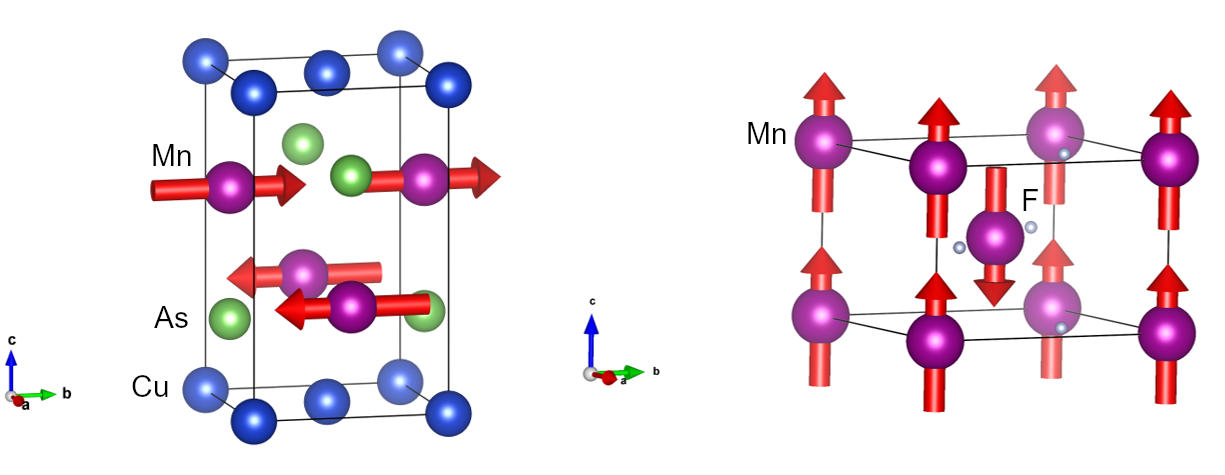
\includegraphics[width=\columnwidth]{figures/ch1/CuMnAs-MnF2.png} \\
\caption{\label{fig:tet-CuMnAs}
Electronic band structure
}
\end{figure}

\section{Exploration of Cu-Mn-As phase space}

% Why are CuMnAs compounds popular?

\begin{figure}
\centering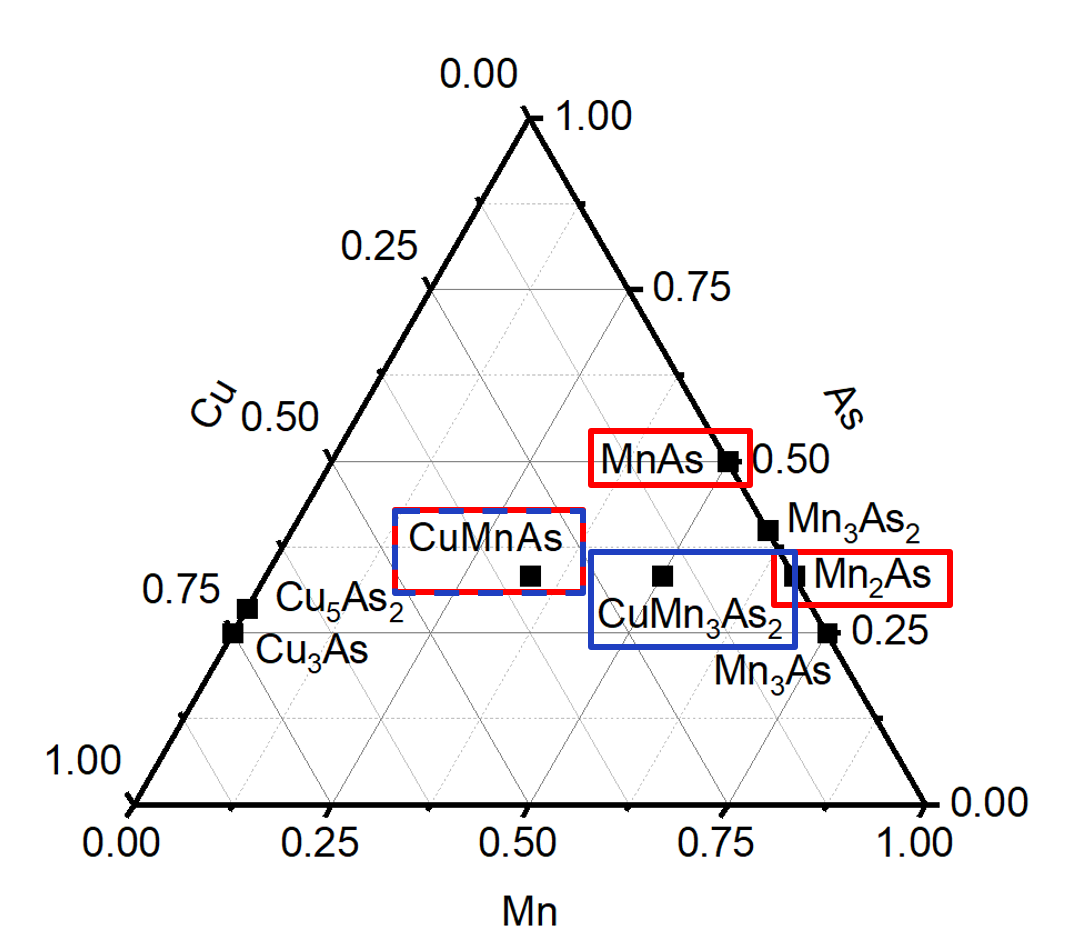
\includegraphics[width=0.8\columnwidth]{figures/ch1/Cu-Mn-As phase diagram.png} \\
\caption{\label{fig:Cu-Mn-As}
Electronic band structure
}
\end{figure}

\begin{figure}
\centering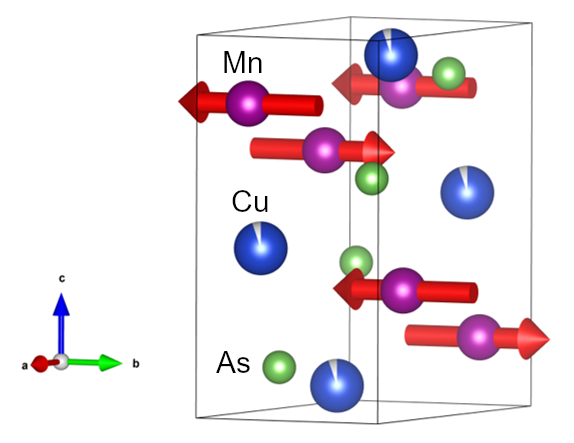
\includegraphics[width=0.5\columnwidth]{figures/ch1/ort-CuMnAs.png} \\
\caption{\label{fig:ort-CuMnAs}
Electronic band structure
}
\end{figure}


% The dual problem


\section{Exchange interactions in Cu$_2$Sb type materials}



%chapter 2
\chapter{Theory of electrical switching in metallic antiferromagnets}

\begin{figure}
\centering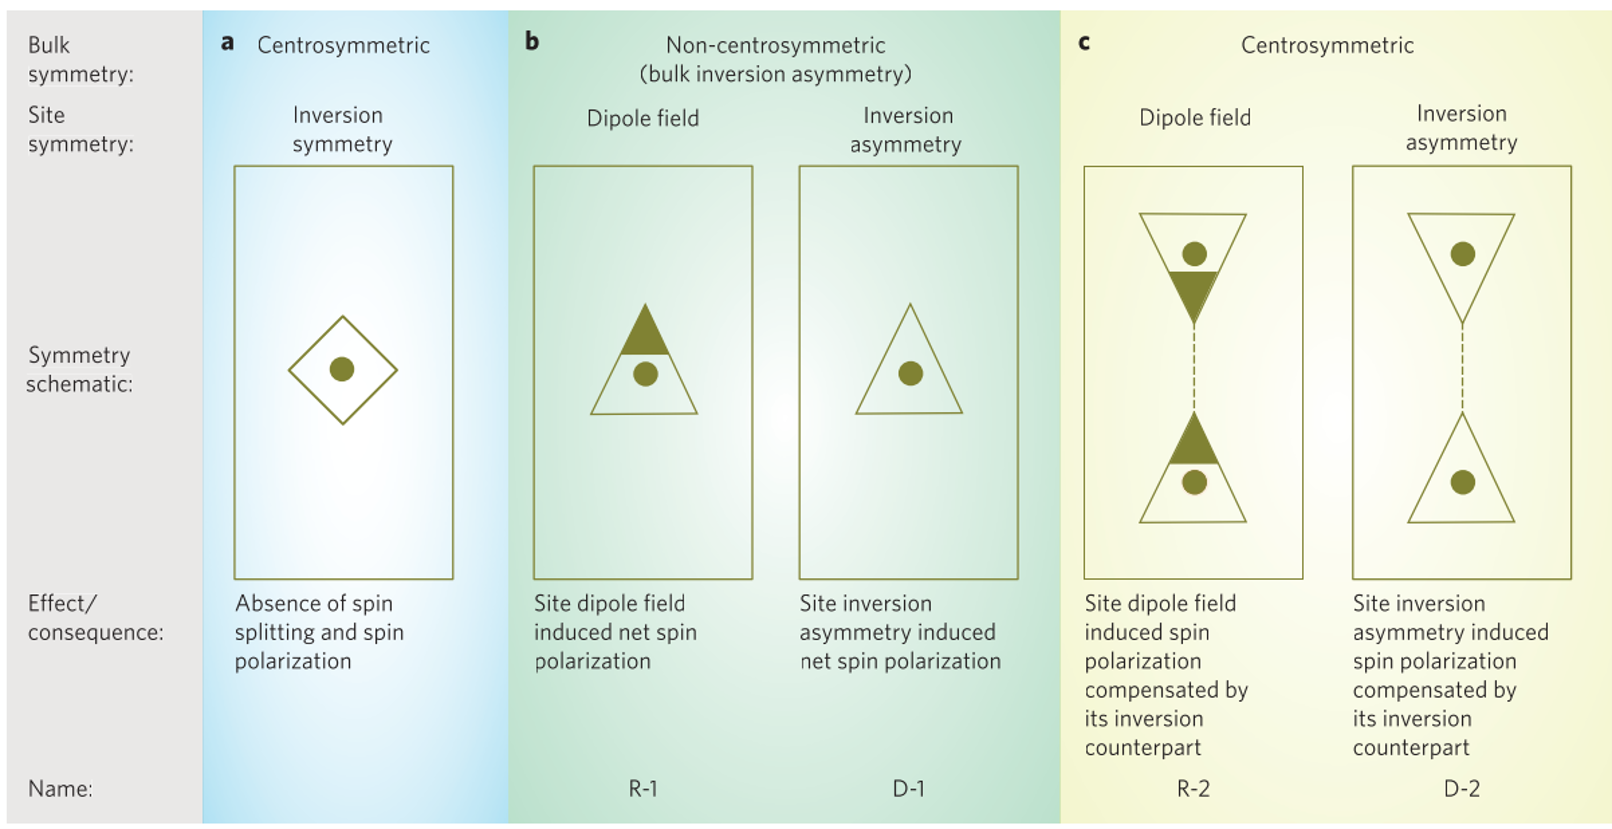
\includegraphics[width=\columnwidth]{figures/ch2/zhang_1.png} \\
\caption{\label{fig:zhang_1}
Electronic band structure
}
\end{figure}

\begin{figure}
\centering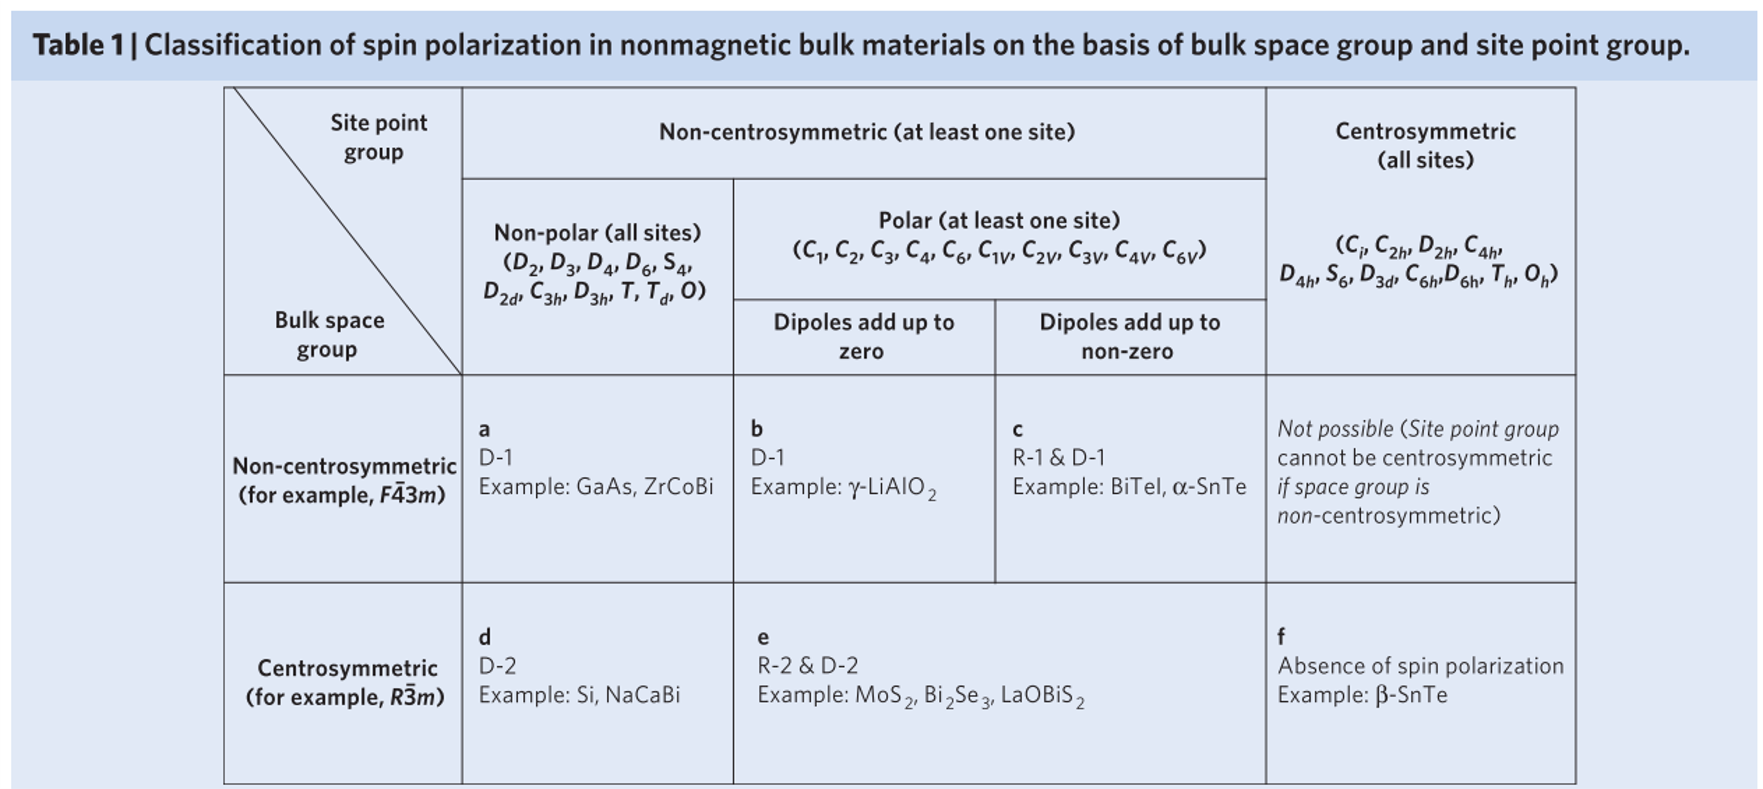
\includegraphics[width=\columnwidth]{figures/ch2/zhang_2.png} \\
\caption{\label{fig:zhang_2}
Electronic band structure
}
\end{figure}

\begin{figure}
\centering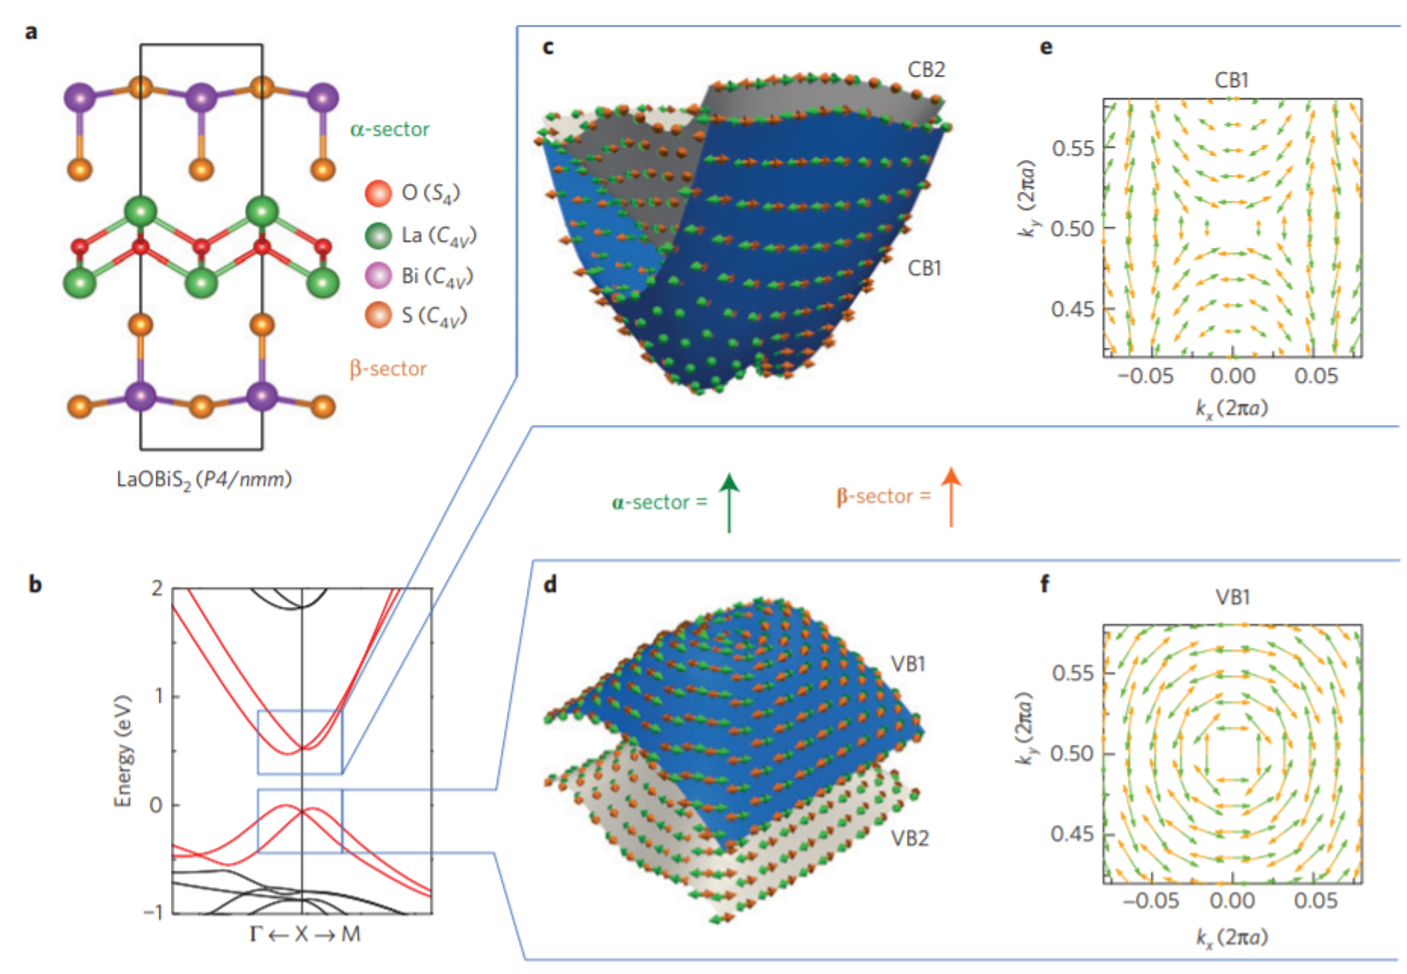
\includegraphics[width=\columnwidth]{figures/ch2/zhang_3.png} \\
\caption{\label{fig:zhang_3}
Electronic band structure
}
\end{figure}

\begin{figure}
\centering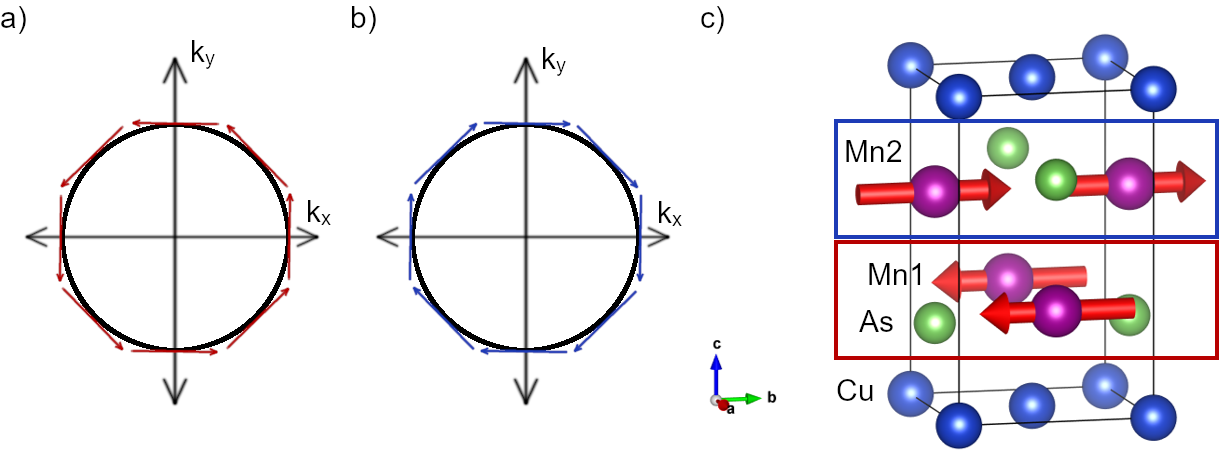
\includegraphics[width=\columnwidth]{figures/ch2/wadley_1.png} \\
\caption{\label{fig:wadley_1}
Electronic band structure
}
\end{figure}

\begin{figure}
\centering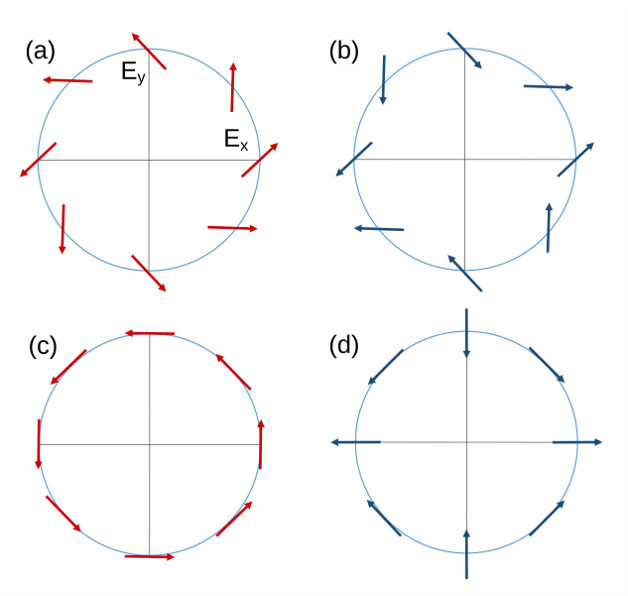
\includegraphics[width=0.7\columnwidth]{figures/ch2/rashba_dresselhaus.png} \\
\caption{\label{fig:rashba_dresselhaus}
Electronic band structure
}
\end{figure}

\begin{figure}
\centering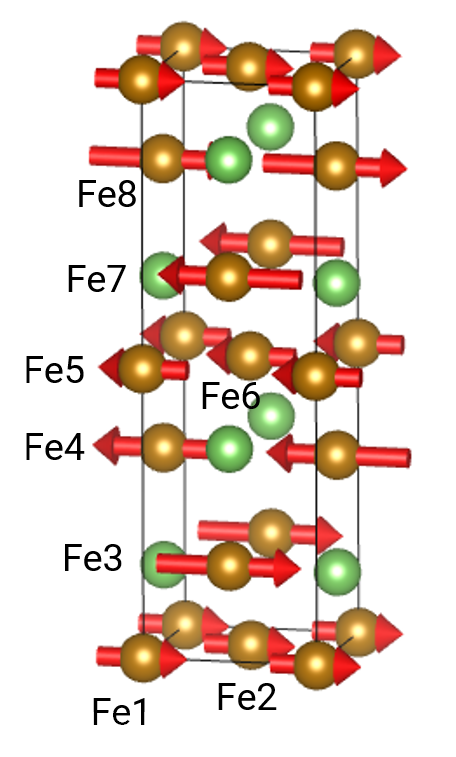
\includegraphics[width=0.3\columnwidth]{figures/ch2/Fe2As.png} \\
\caption{\label{fig:Fe2As}
Electronic band structure
}
\end{figure}

\begin{figure}
\centering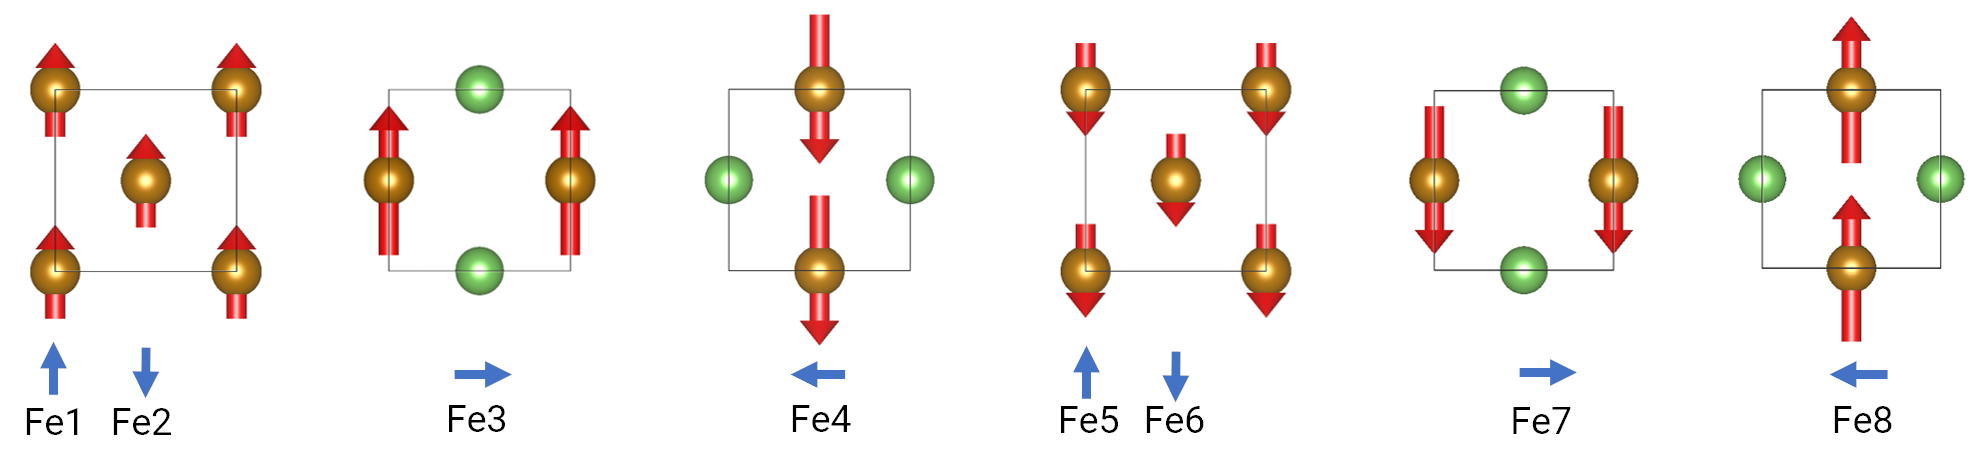
\includegraphics[width=\columnwidth]{figures/ch2/fieldlike_torque_Fe2As.png} \\
\caption{\label{fig:fieldlike_torque_Fe2As}
Electronic band structure
}
\end{figure}

\begin{figure}
\centering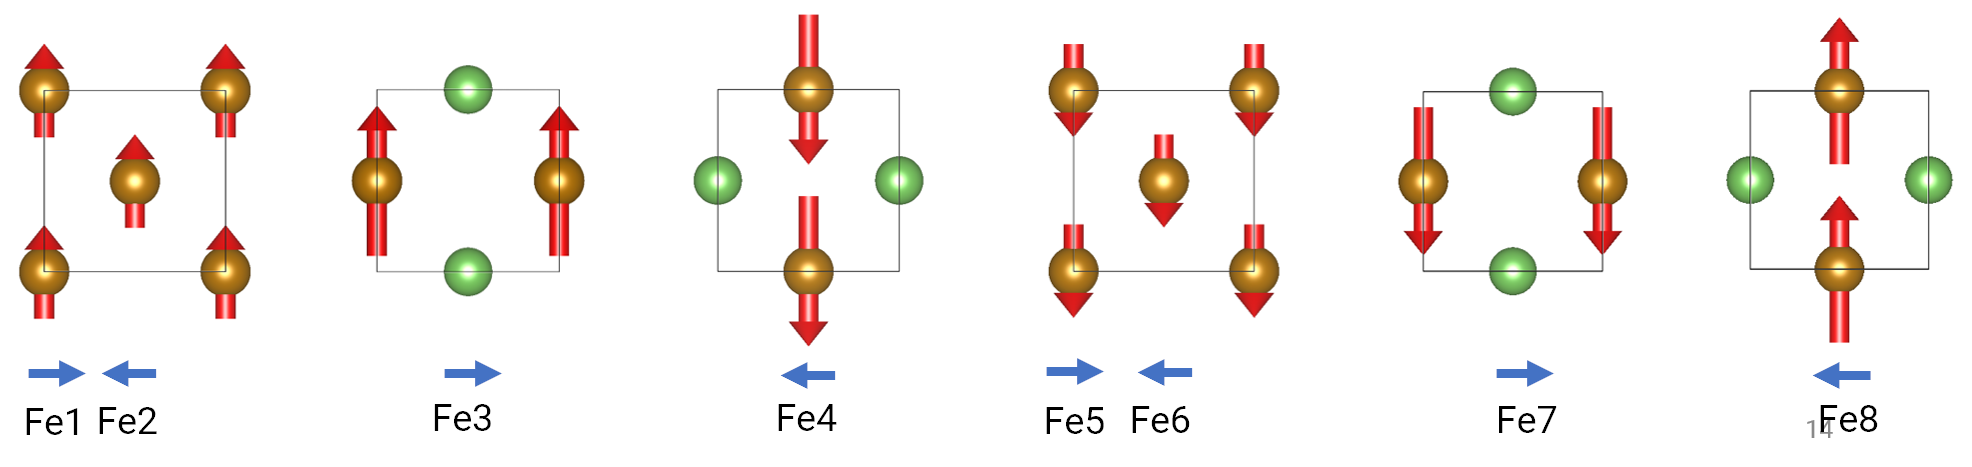
\includegraphics[width=\columnwidth]{figures/ch2/antidamping_torque_Fe2As.png} \\
\caption{\label{fig:antidamping_torque_Fe2As}
Electronic band structure
}
\end{figure}

\Blindtext[6]

%chapter 3
\chapter{Magnetic structure refinement from neutron diffraction measurements}

\begin{figure}
\centering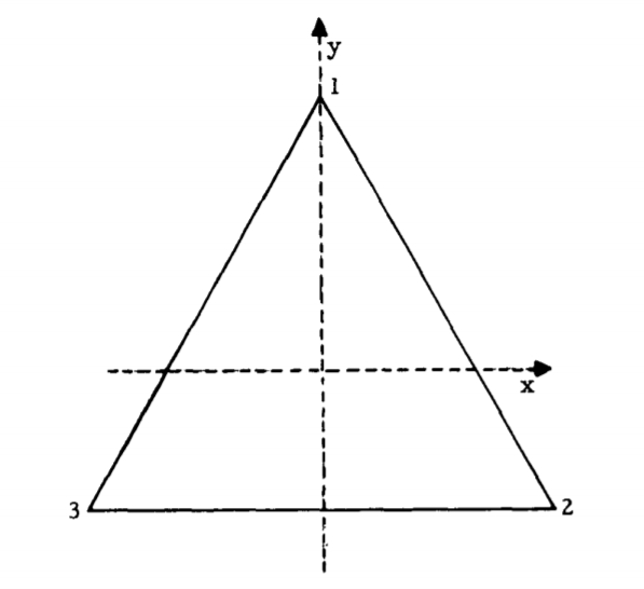
\includegraphics[width=0.5\columnwidth]{figures/ch3/C3v.png} \\
\caption{\label{fig:C3v}
Electronic band structure
}
\end{figure}

\begin{figure}
\centering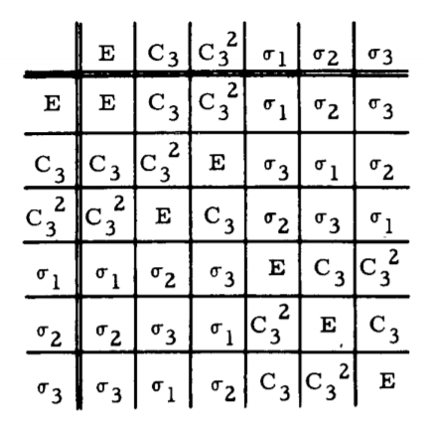
\includegraphics[width=0.5\columnwidth]{figures/ch3/group_multiplication_table_C3v.png} \\
\caption{\label{fig:gmt_C3v}
Electronic band structure
}
\end{figure}

\begin{figure}
\centering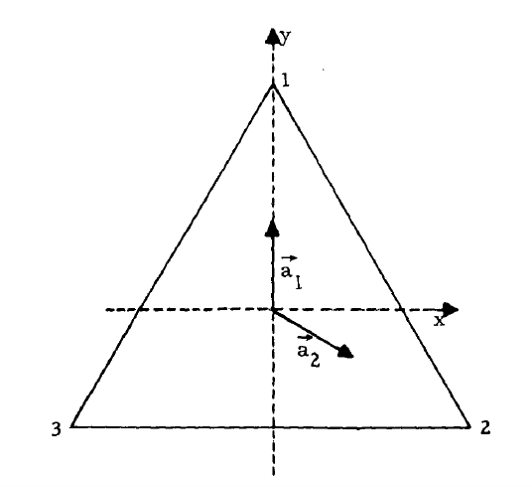
\includegraphics[width=0.5\columnwidth]{figures/ch3/C3v_a1_a2.png} \\
\caption{\label{fig:C3v_a1_a2}
Electronic band structure
}
\end{figure}

\begin{figure}
\centering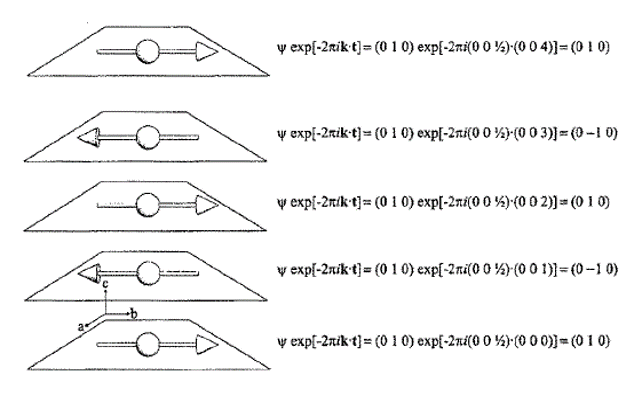
\includegraphics[width=\columnwidth]{figures/ch3/propagation_vector.png} \\
\caption{\label{fig:propagation_vector}
Electronic band structure
}
\end{figure}

\begin{figure}
\centering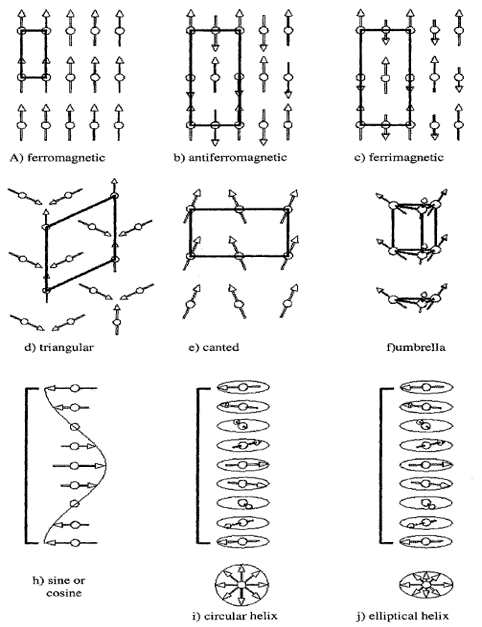
\includegraphics[width=\columnwidth]{figures/ch3/mag_structures_single_k.png} \\
\caption{\label{fig:mag_structures_single_k}
Electronic band structure
}
\end{figure}

\begin{figure}
\centering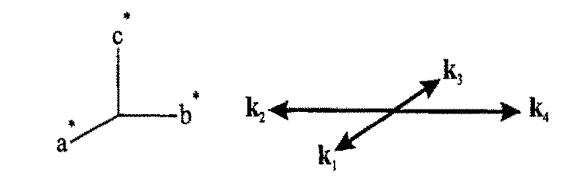
\includegraphics[width=0.7\columnwidth]{figures/ch3/star_of_propagation_vector_k.png} \\
\caption{\label{fig:star}
Electronic band structure
}
\end{figure}

\begin{figure}
\centering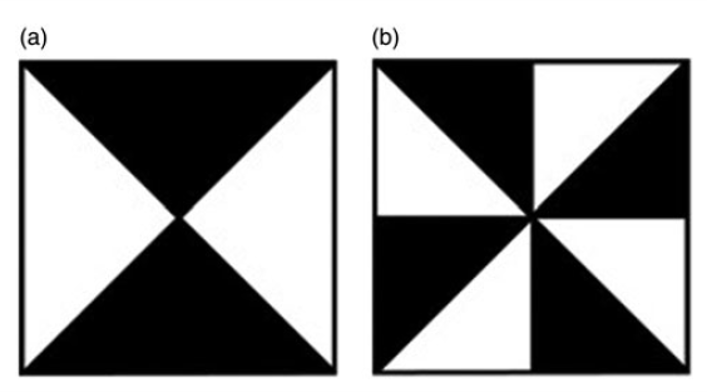
\includegraphics[width=0.5\columnwidth]{figures/ch3/symmetry_based_analysis.png} \\
\caption{\label{fig:symmetry_based_analysis}
Electronic band structure
}
\end{figure}

\Blindtext[6]

%chapter 4
\chapter{Materials synthesis and characterization}

This is a citation to~\cite{Walker2015} and~\cite{Hager2006}.

\begin{figure}
\centering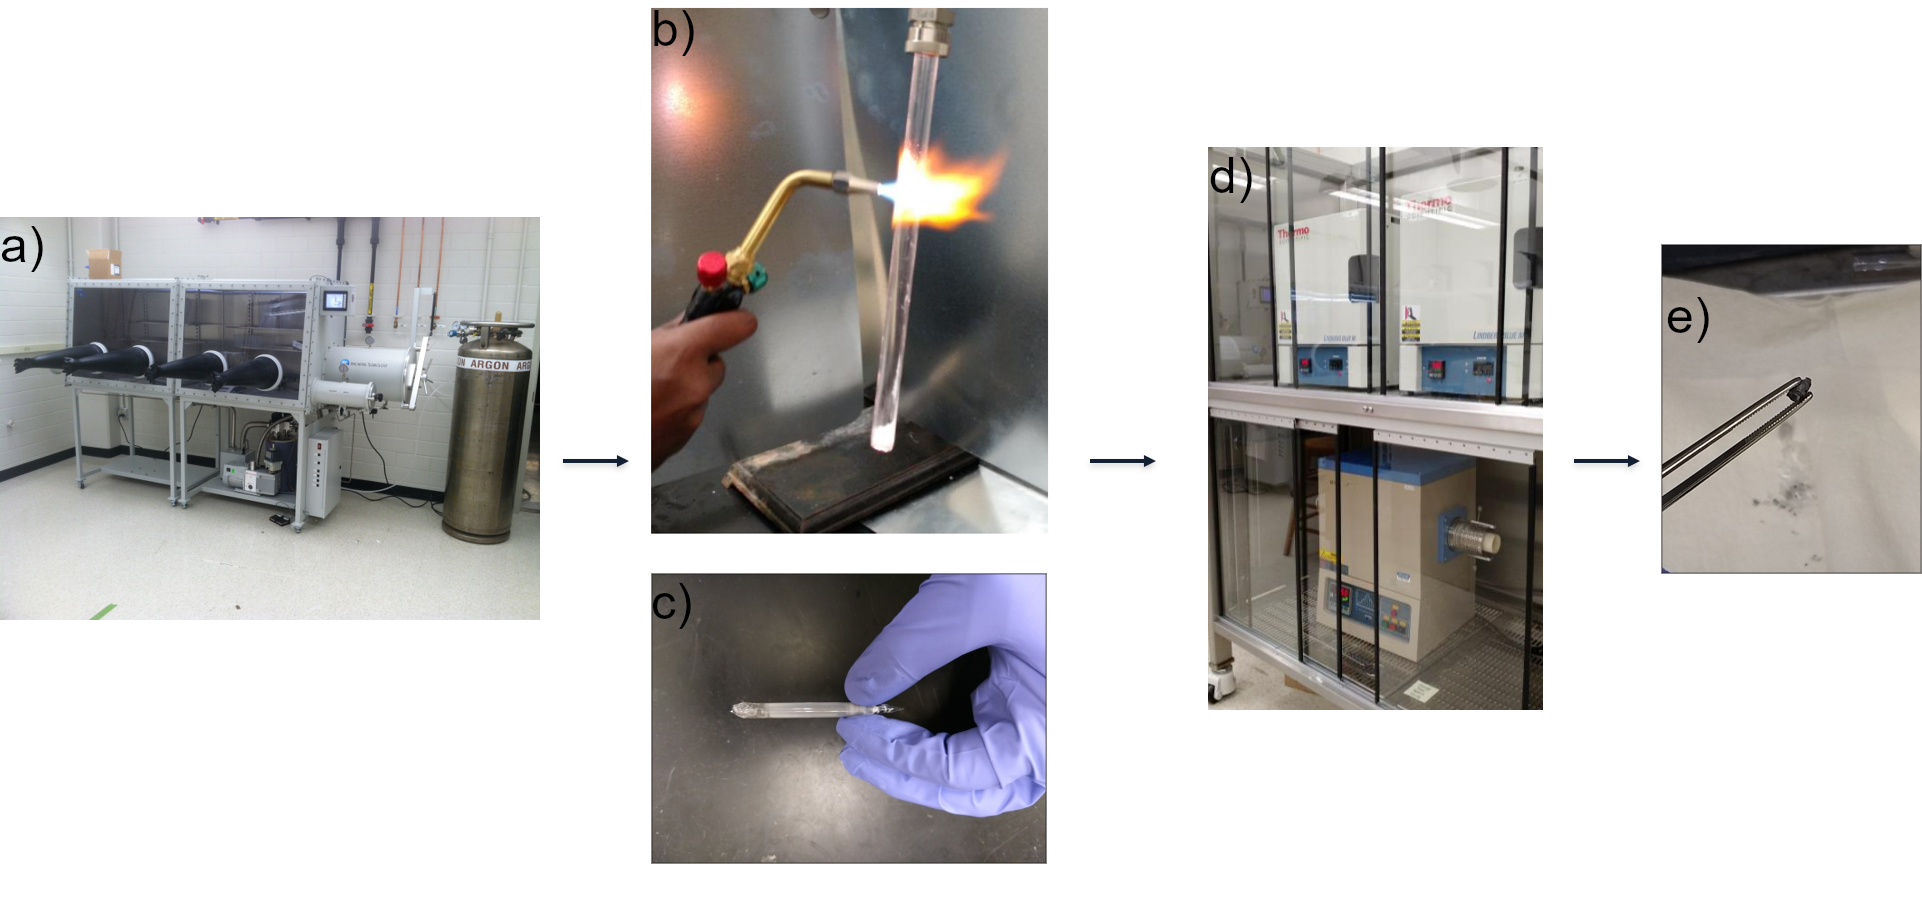
\includegraphics[width=\columnwidth]{figures/ch4/synthesis_procedure.png} \\
\caption{\label{fig:synthesis_procedure}
Electronic band structure
}
\end{figure}

%chapter 5
\chapter{Discovery and magnetic frustration of hexagonal Cu$_{0.82}$Mn$_{1.18}$As}

\begin{figure}
\centering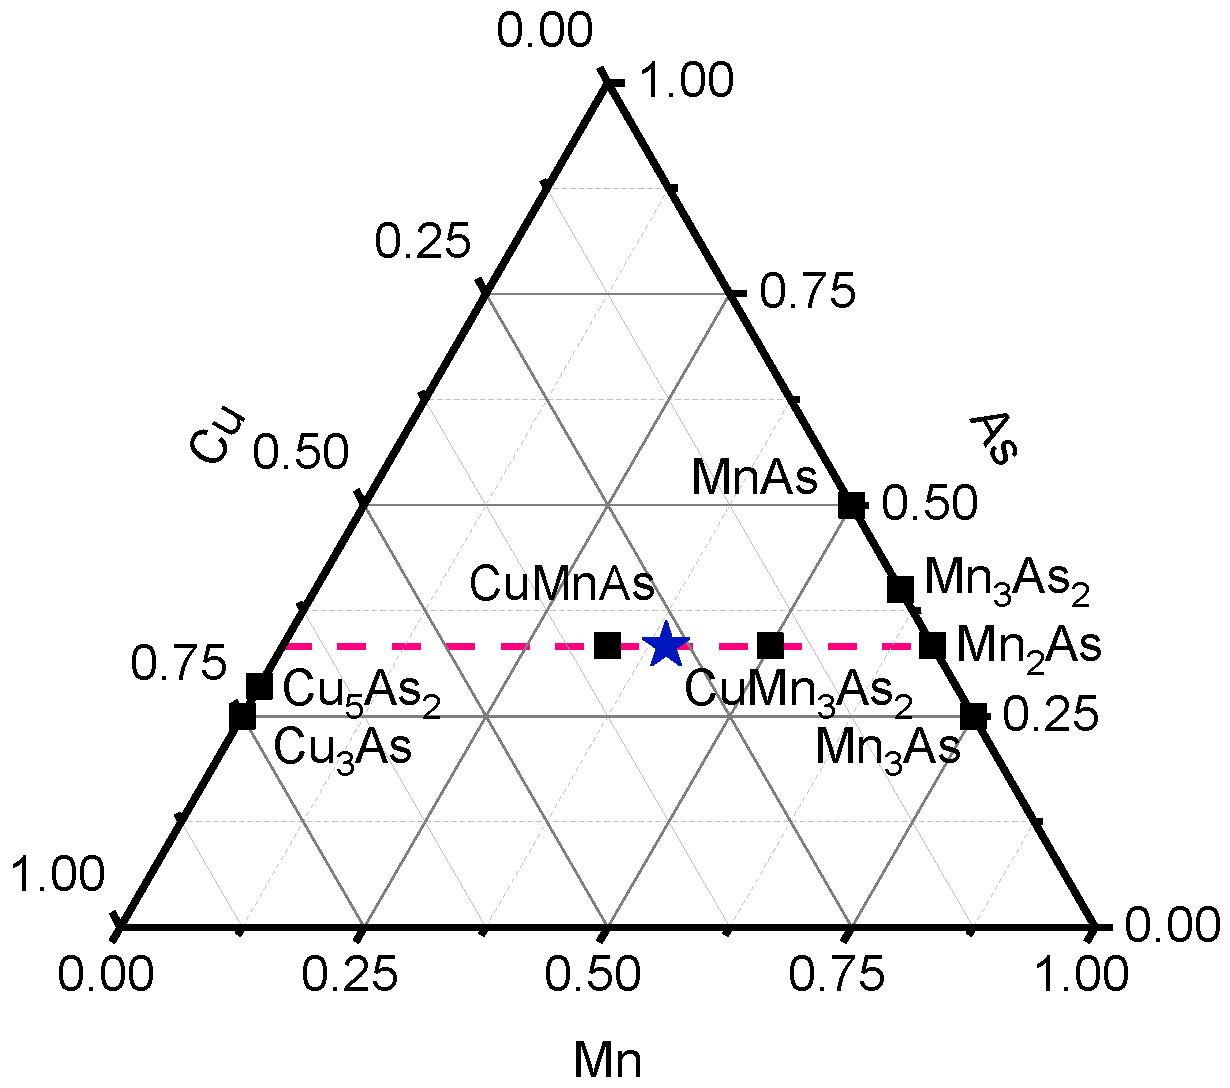
\includegraphics[width=\columnwidth]{figures/ch5/phase_diagram_cropped.pdf} \\
\caption{\label{fig:phase_diagram}
Electronic band structure
}
\end{figure}

\begin{figure}
\centering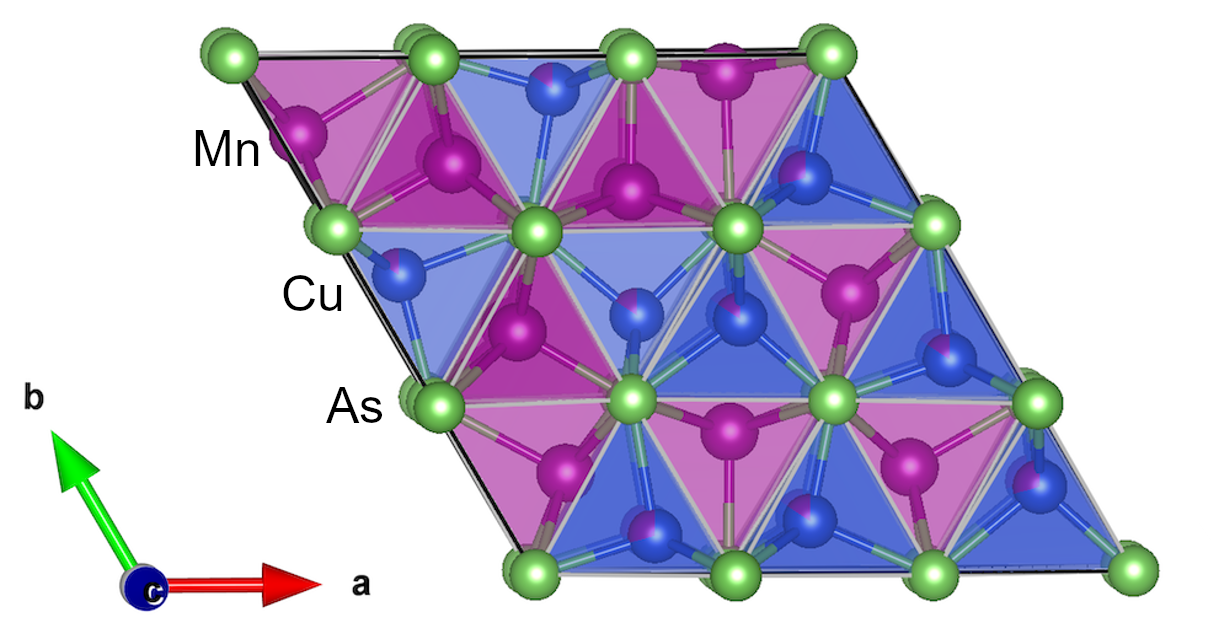
\includegraphics[width=\columnwidth]{figures/ch5/CuMnAs_chemical_structure.png} \\
\caption{\label{fig:chemical_structure}
Electronic band structure
}
\end{figure}

\begin{figure}
\centering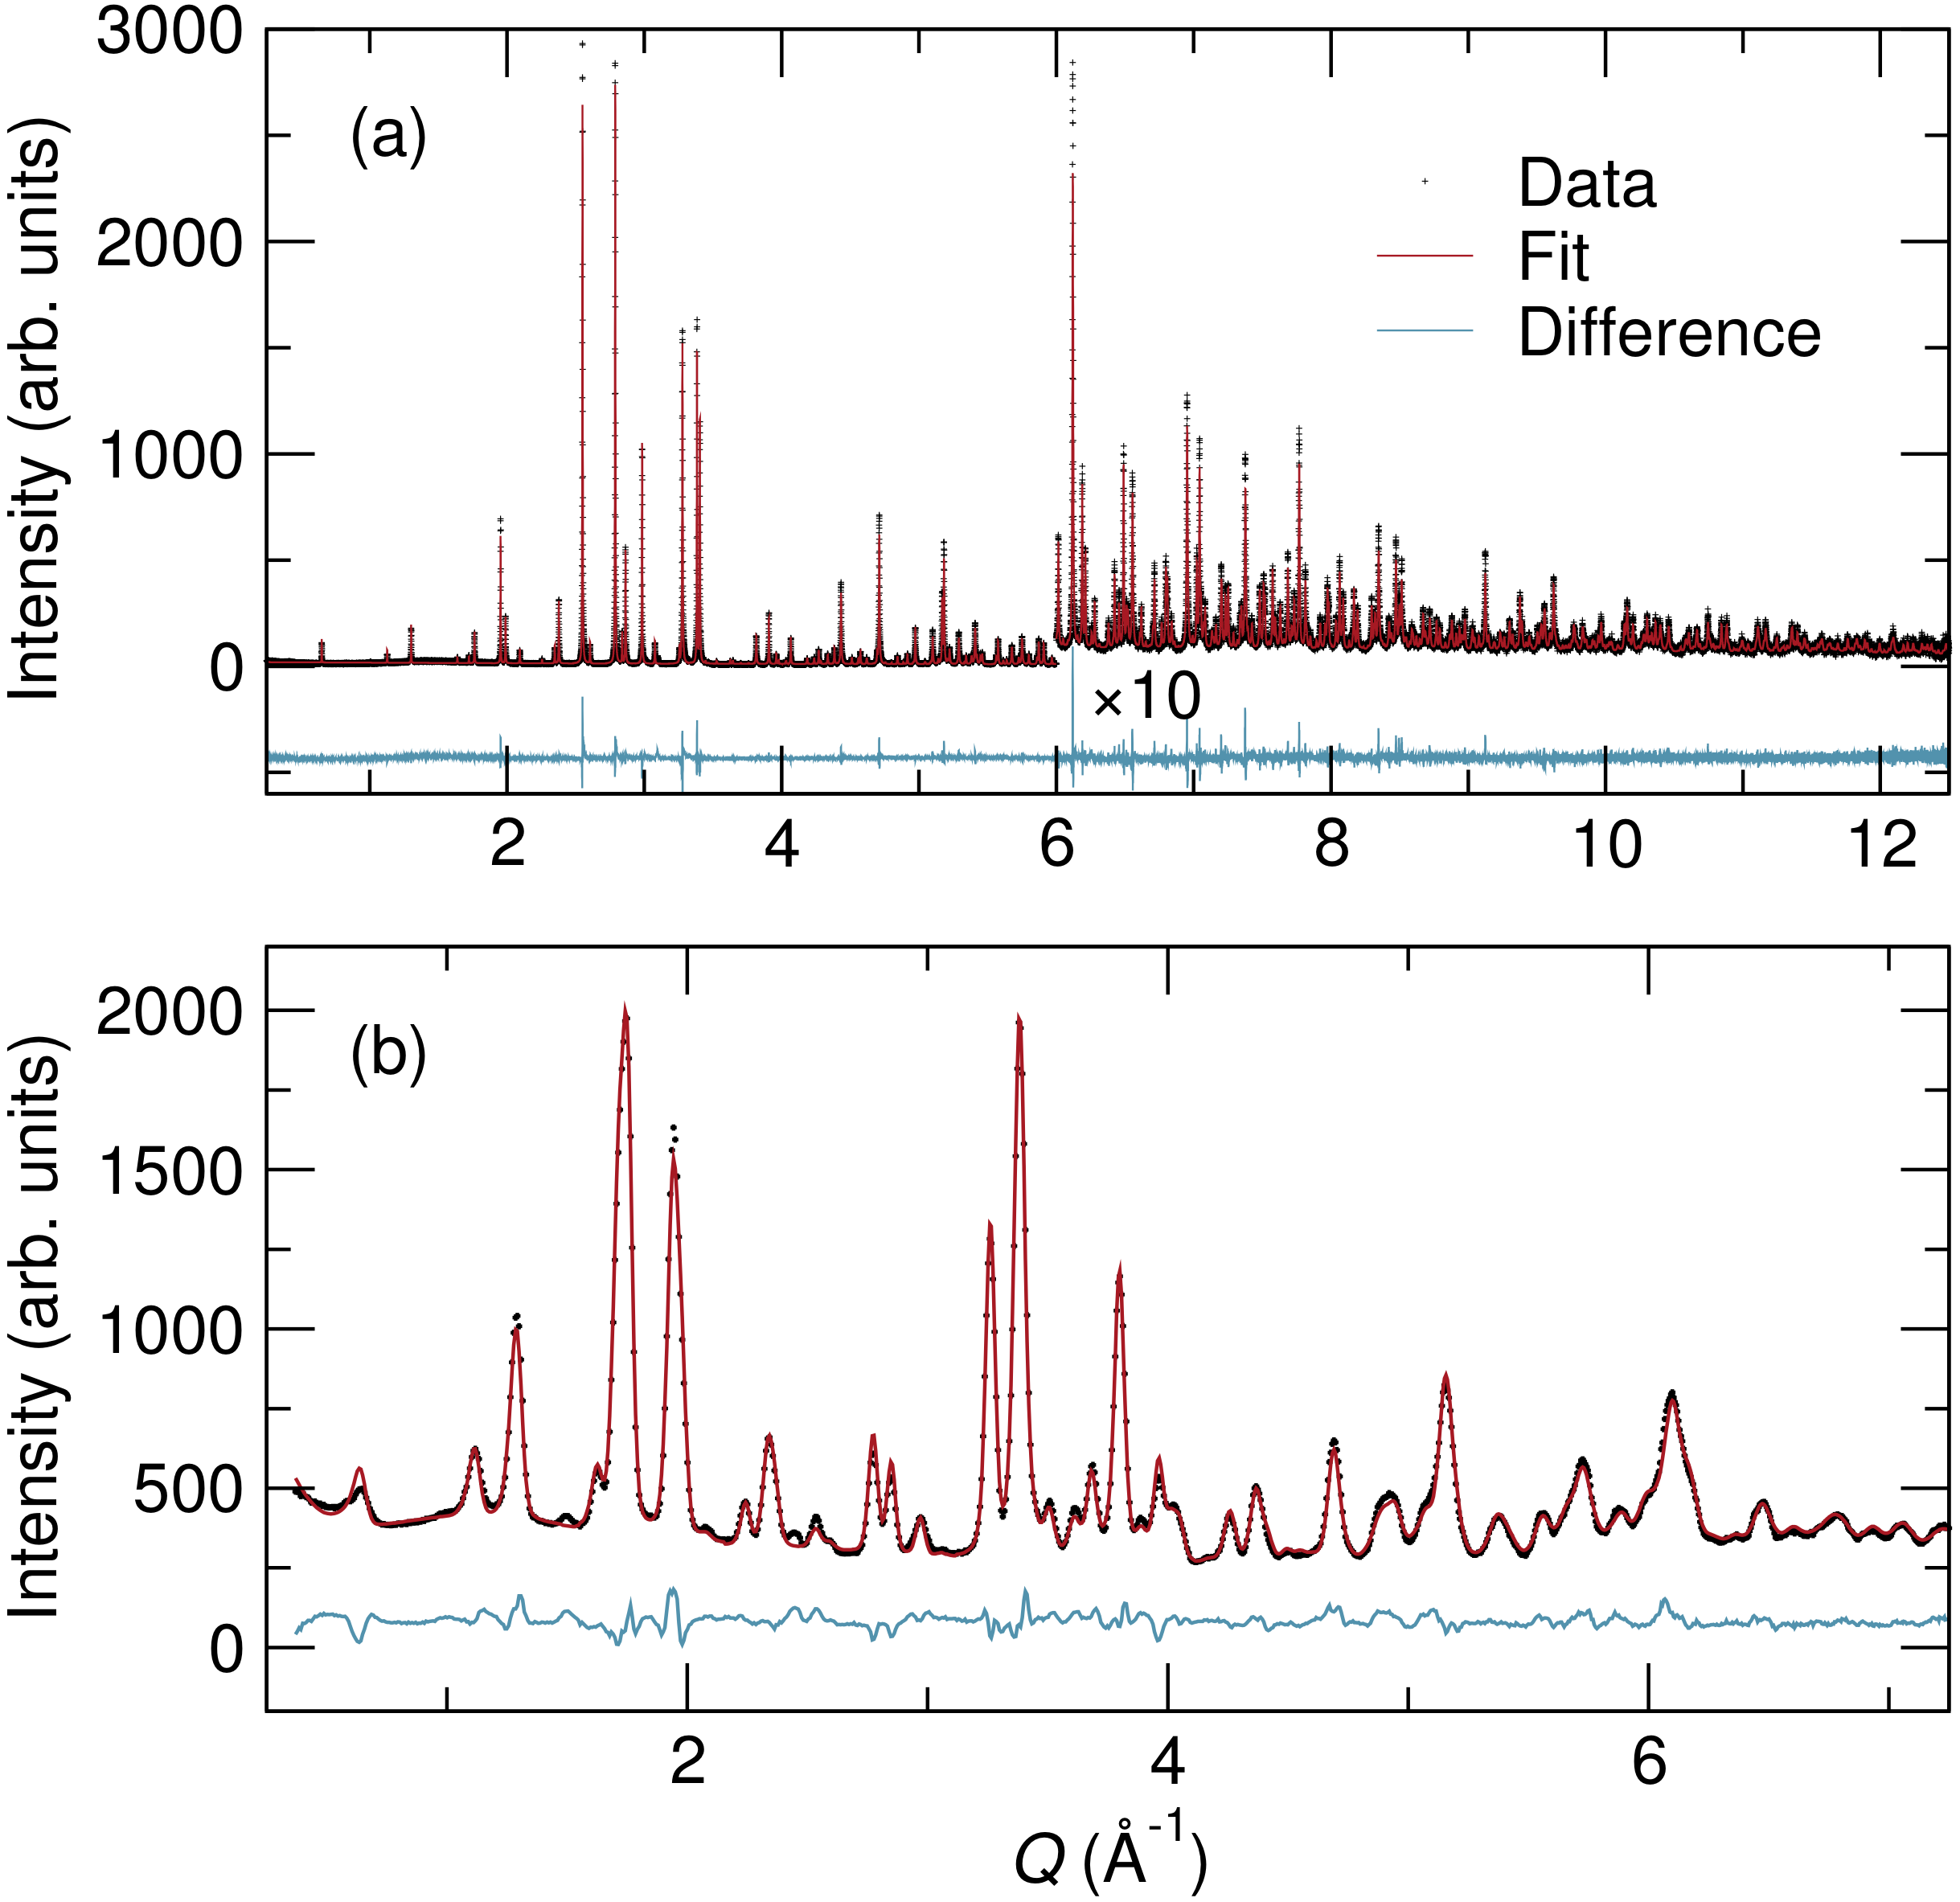
\includegraphics[width=\columnwidth]{figures/ch5/h-cumnas_11bm_100k_wand_400k_combine.png} \\
\caption{\label{fig:11BM_WAND}
Electronic band structure
}
\end{figure}

\begin{figure}
\centering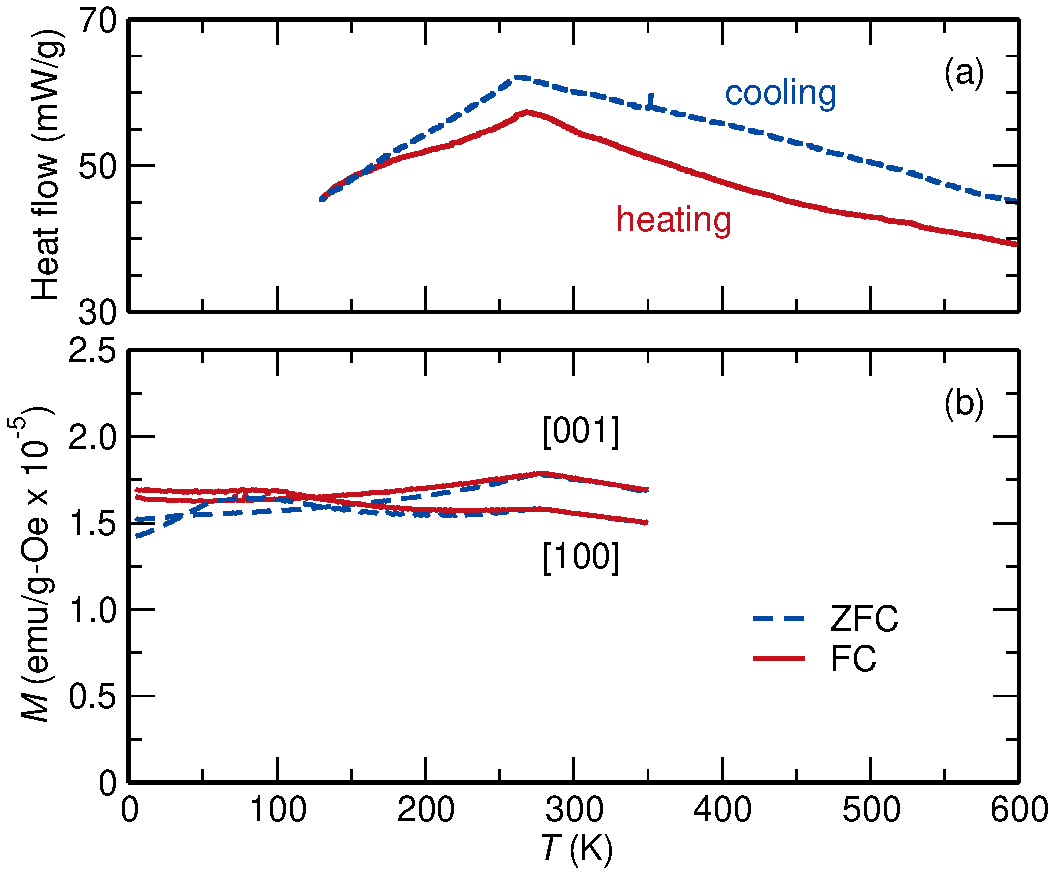
\includegraphics[width=\columnwidth]{figures/ch5/dsc-mpms_norm_cropped.pdf} \\
\caption{\label{fig:dsc_mpms}
Electronic band structure
}
\end{figure}

\begin{figure}
\centering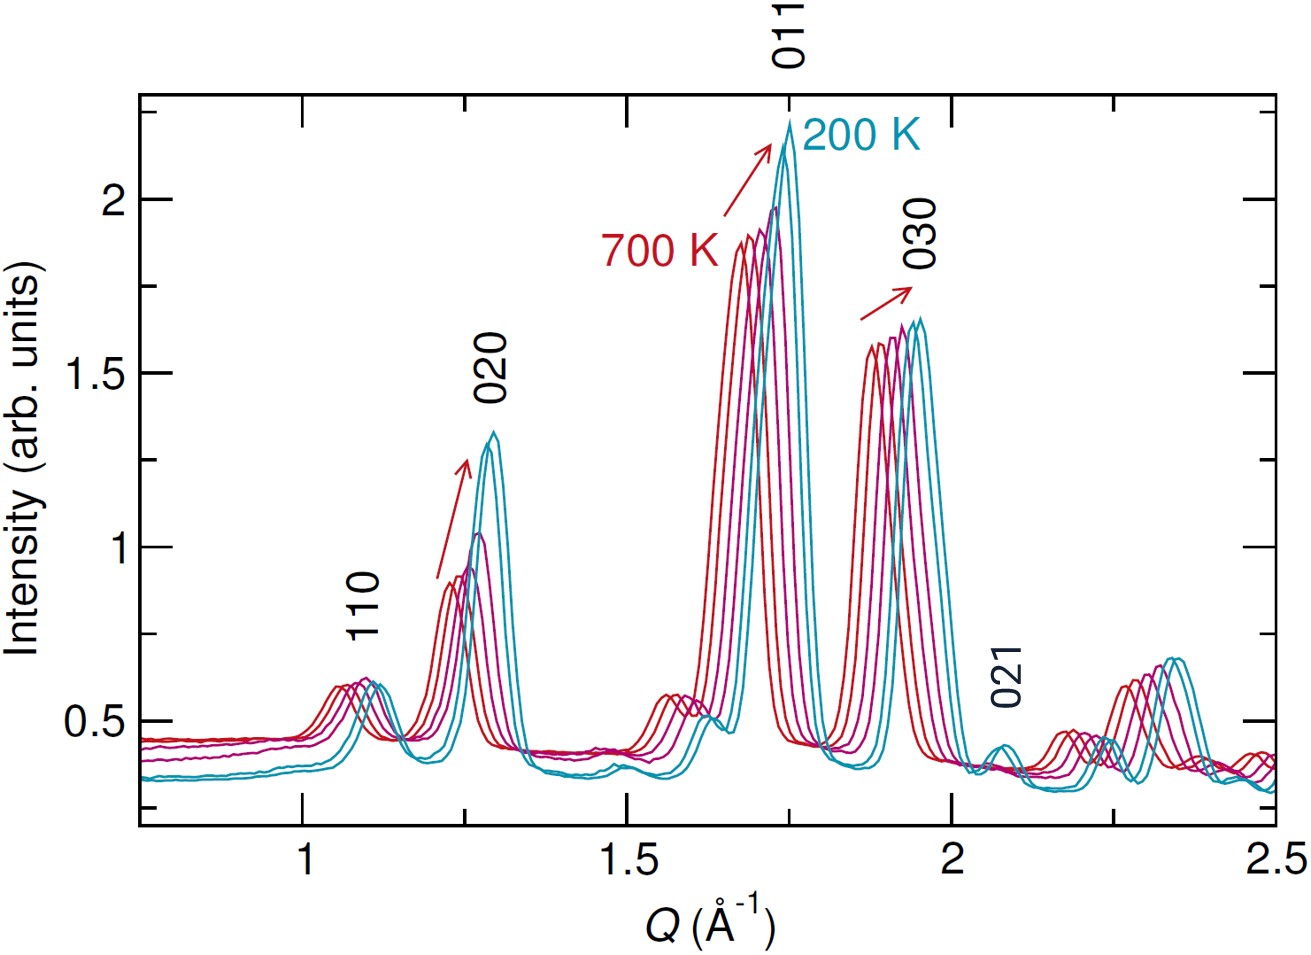
\includegraphics[width=\columnwidth]{figures/ch5/WAND_data.png} \\
\caption{\label{fig:WAND_data}
Electronic band structure
}
\end{figure}

\begin{figure}
\centering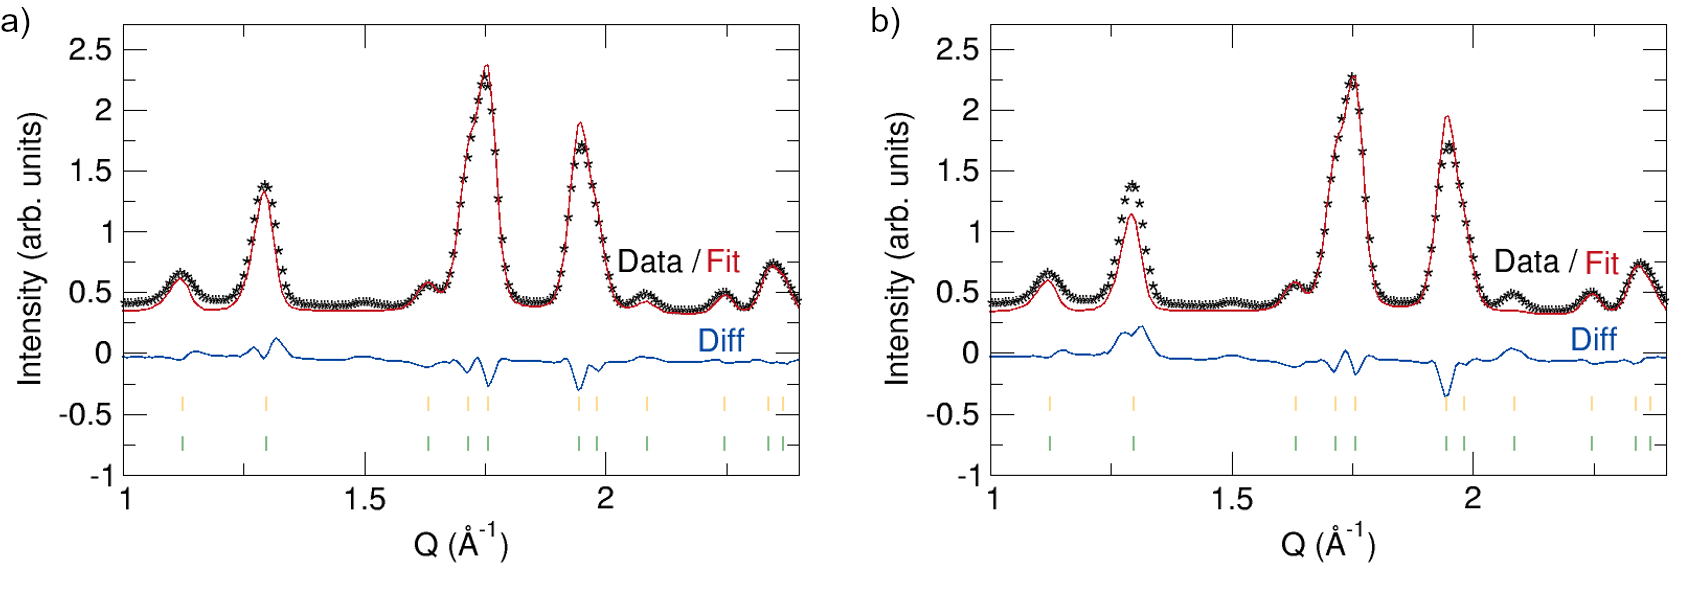
\includegraphics[width=\columnwidth]{figures/ch5/wand_refinement.png} \\
\caption{\label{fig:wand_refinement}
Electronic band structure
}
\end{figure}

\begin{figure}
\centering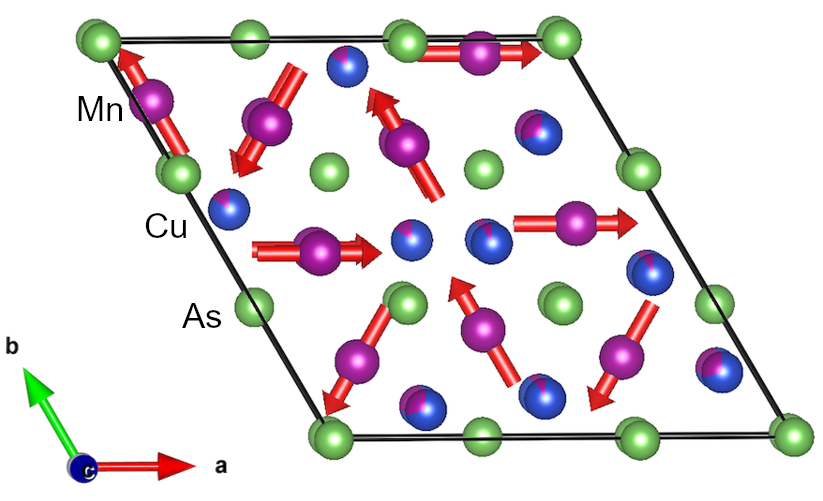
\includegraphics[width=\columnwidth]{figures/ch5/CuMnAs_magnetic_structure.png} \\
\caption{\label{fig:CuMnAs_magnetic_structure}
Electronic band structure
}
\end{figure}

\begin{figure}
\centering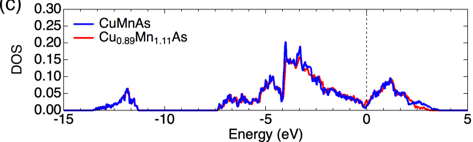
\includegraphics[width=\columnwidth]{figures/ch5/DOS_CuMnAs.png} \\
\caption{\label{fig:DOS}
Electronic band structure
}
\end{figure}

\begin{figure}
\centering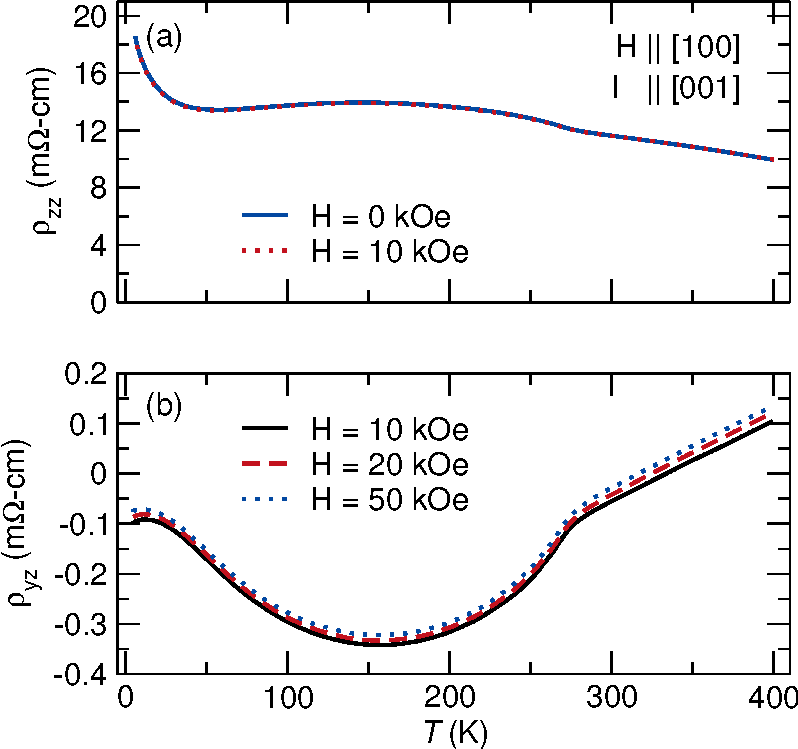
\includegraphics[width=\columnwidth]{figures/ch5/resistivity_data_hall_cropped.pdf} \\
\caption{\label{fig:resistivity}
Electronic band structure
}
\end{figure}

\Blindtext[6]

%chapter 6
\chapter{Two step magnetic ordering in monoclinic Mn$_3$As$_2$}

\begin{figure}
\centering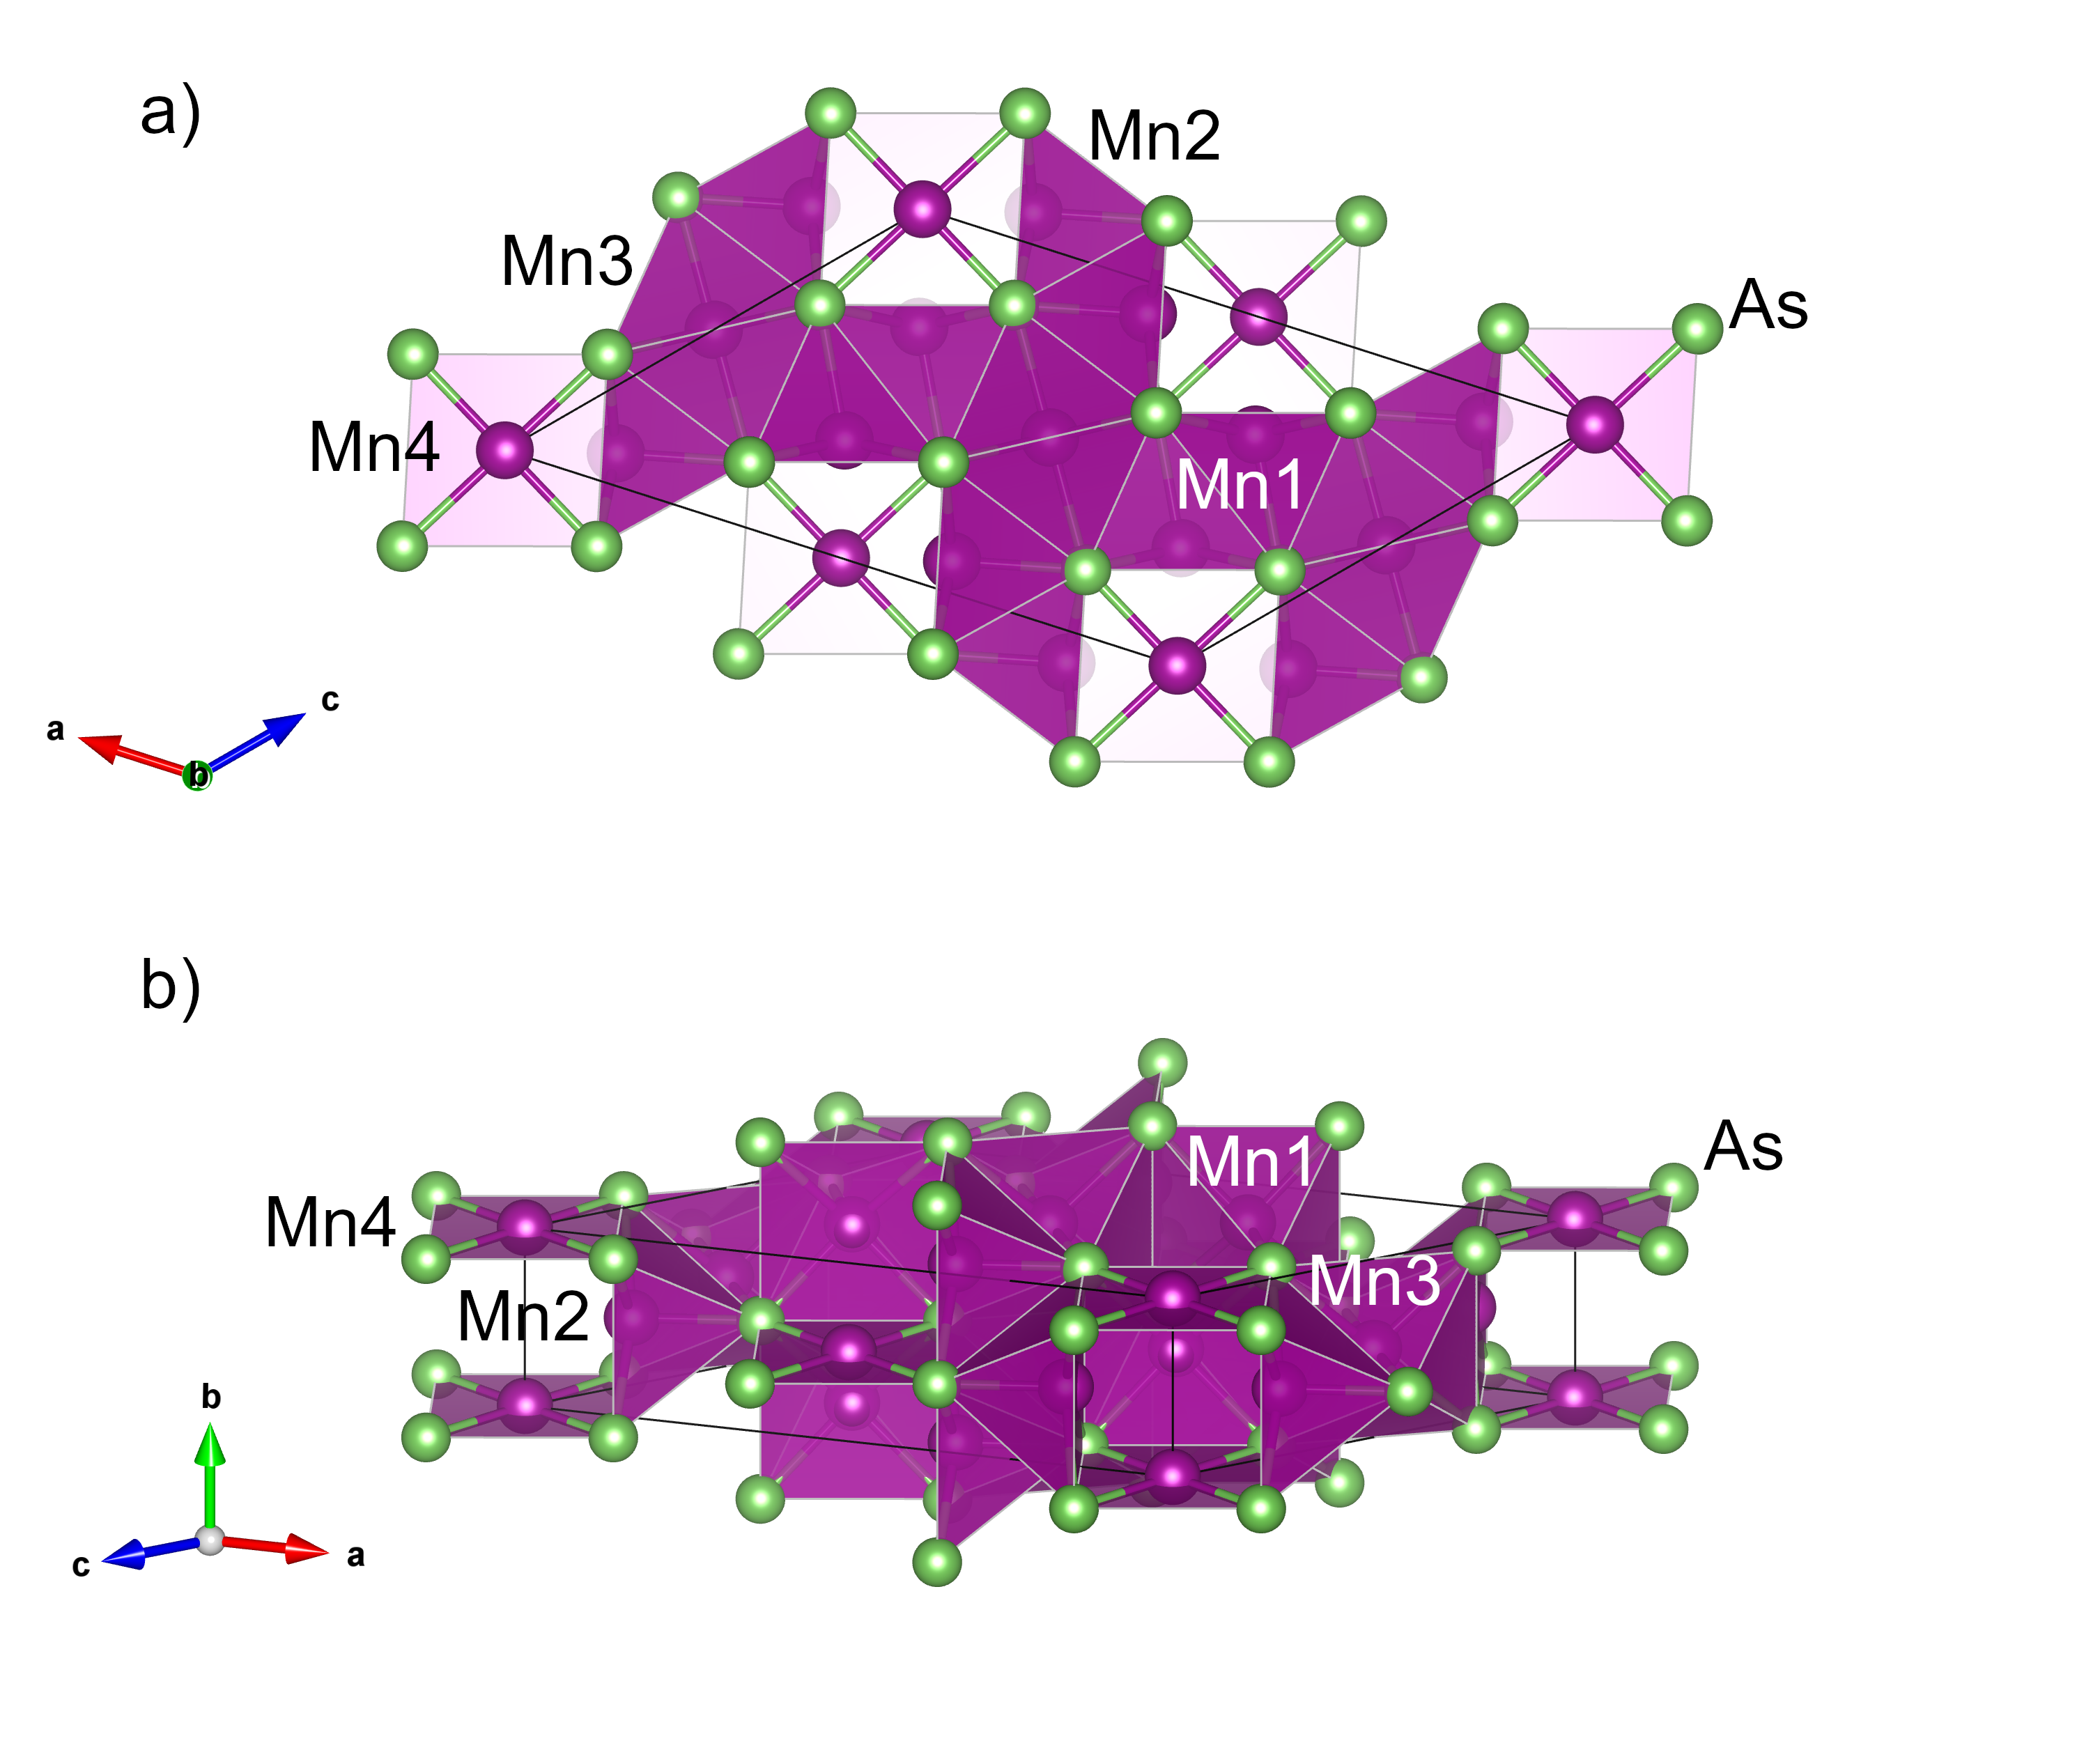
\includegraphics[width=\columnwidth]{figures/ch6/monoclinic_Mn3As2_75510.png} \\
\caption{\label{fig:Mn3As2}
Electronic band structure
}
\end{figure}

\begin{figure}
\centering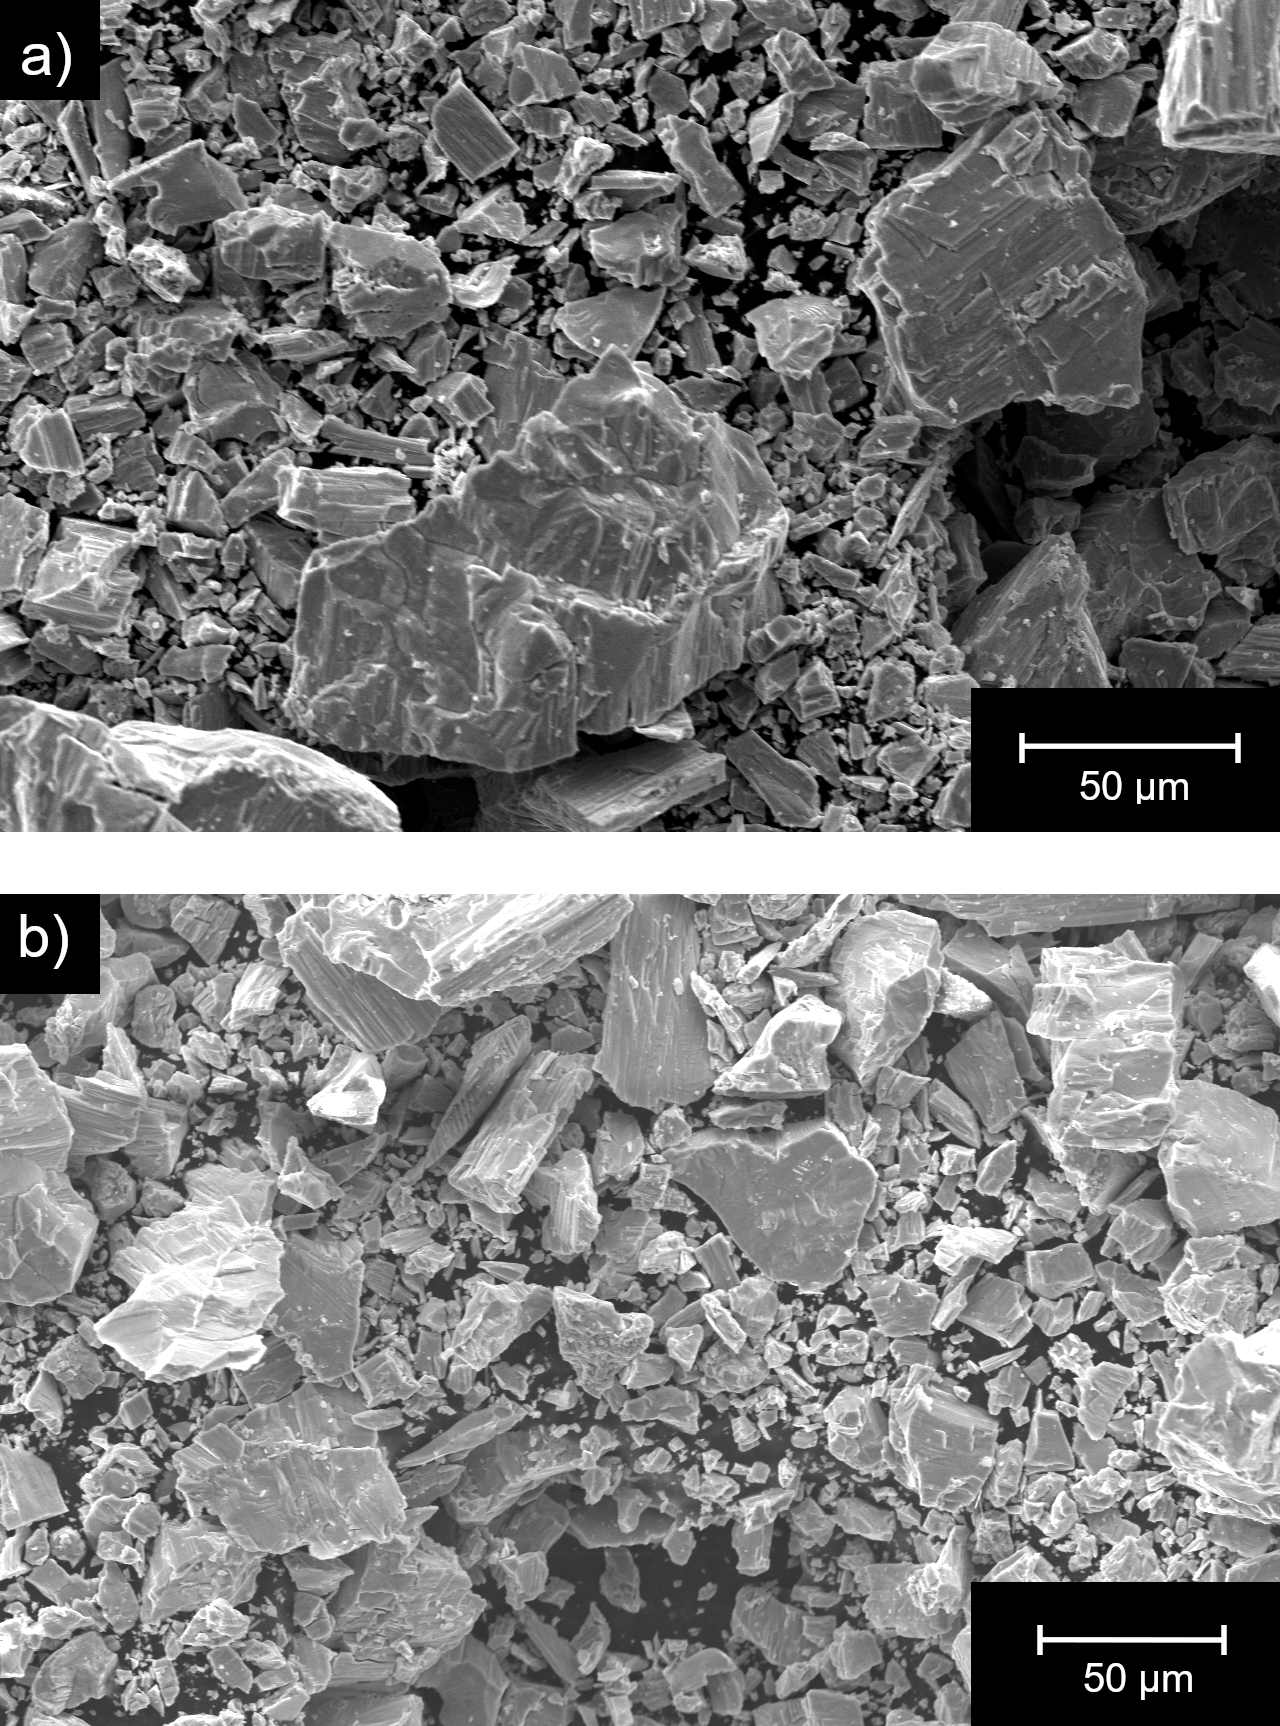
\includegraphics[width=0.5\columnwidth]{figures/ch6/Mn3As2_SEM_image.png} \\
\caption{\label{fig:Mn3As2_SEM}
Electronic band structure
}
\end{figure}

\begin{figure}
\centering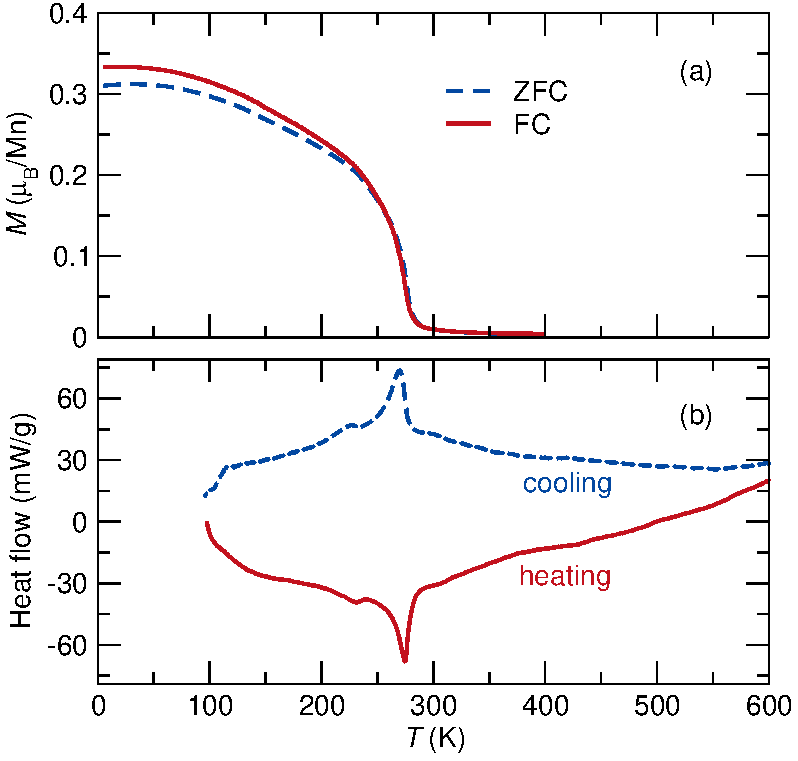
\includegraphics[width=\columnwidth]{figures/ch6/FC_ZFC_DSC_Mn3As2_cropped.pdf} \\
\caption{\label{fig:Mn3As2_FC_ZFC_DSC}
Electronic band structure
}
\end{figure}

\begin{figure}
\centering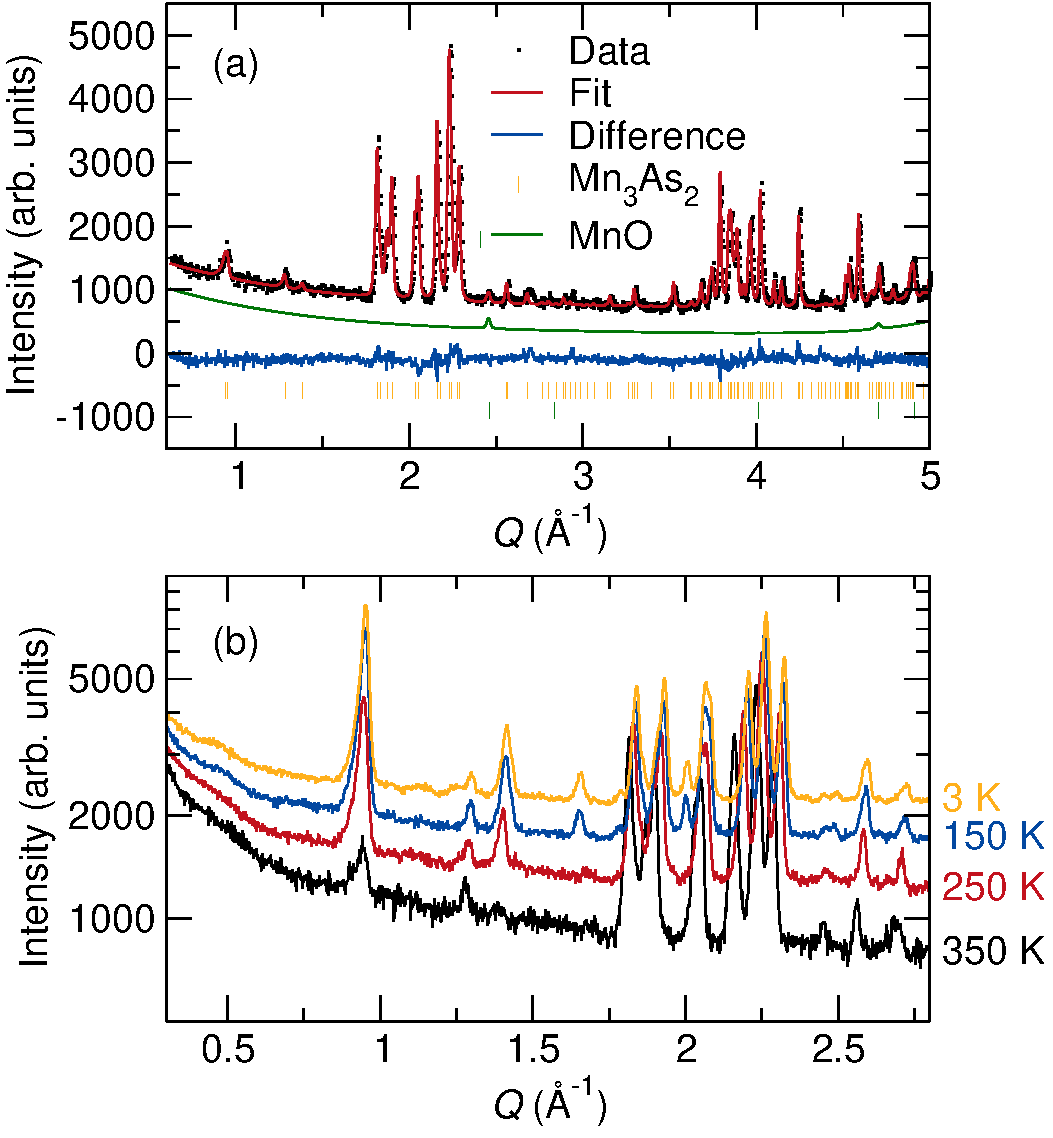
\includegraphics[width=\columnwidth]{figures/ch6/350K_rietveld_diff_temp_NPD_cropped.pdf} \\
\caption{\label{fig:350K}
Electronic band structure
}
\end{figure}

\begin{figure}
\centering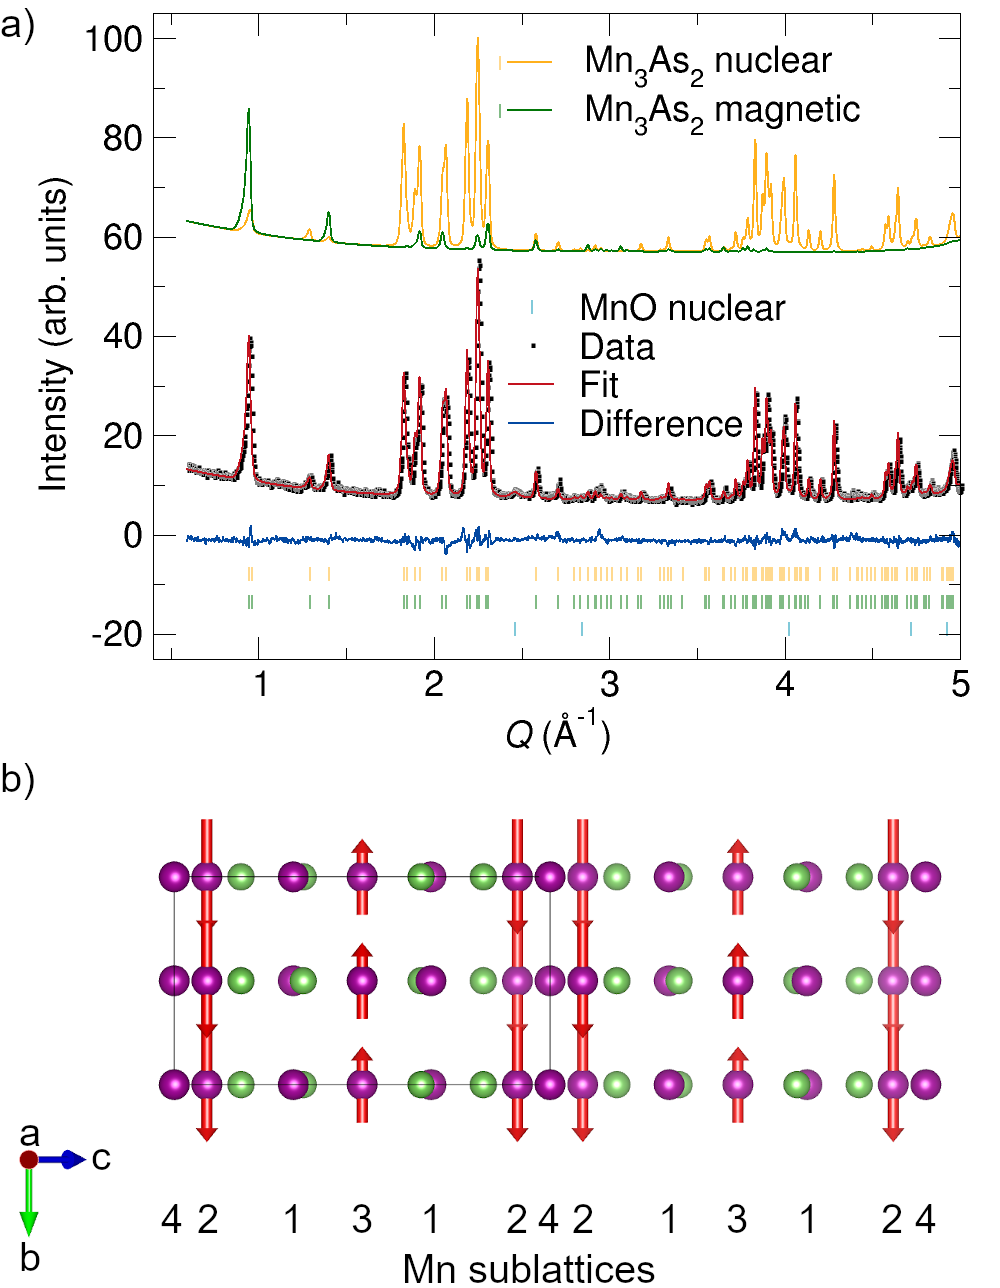
\includegraphics[width=\columnwidth]{figures/ch6/250K_mag_structure.png} \\
\caption{\label{fig:250K}
Electronic band structure
}
\end{figure}


\begin{figure}
\centering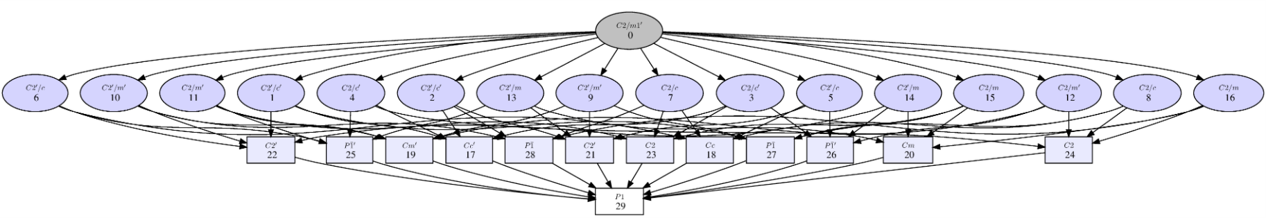
\includegraphics[width=\columnwidth]{figures/ch6/graph_of_subgraphs_3K.png} \\
\caption{\label{fig:subgraphs}
Electronic band structure
}
\end{figure}

\begin{figure}
\centering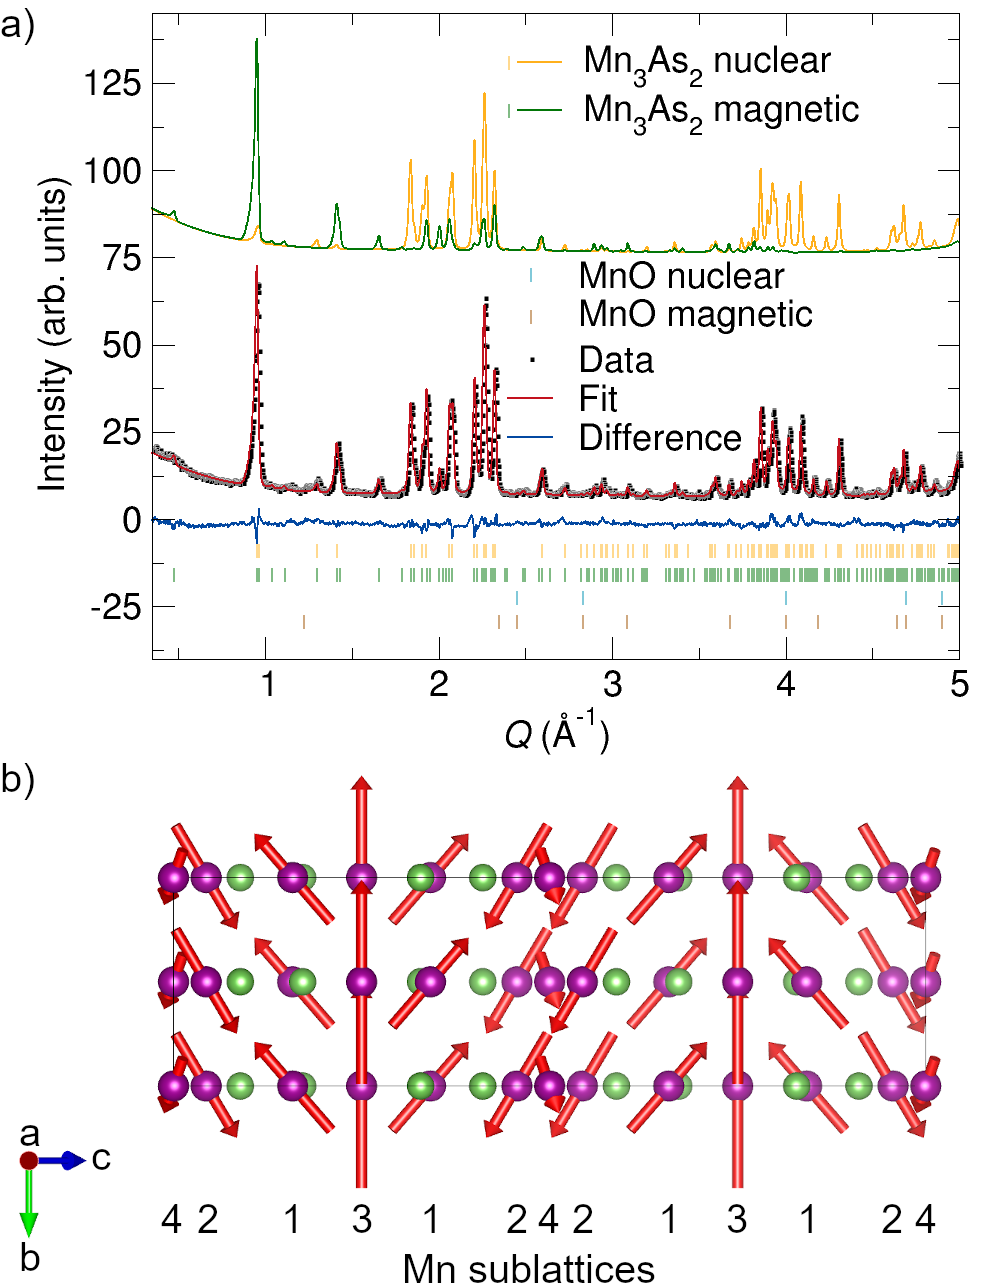
\includegraphics[width=\columnwidth]{figures/ch6/3K_mag_structure.png} \\
\caption{\label{fig:3K}
Electronic band structure
}
\end{figure}


\begin{figure}
\centering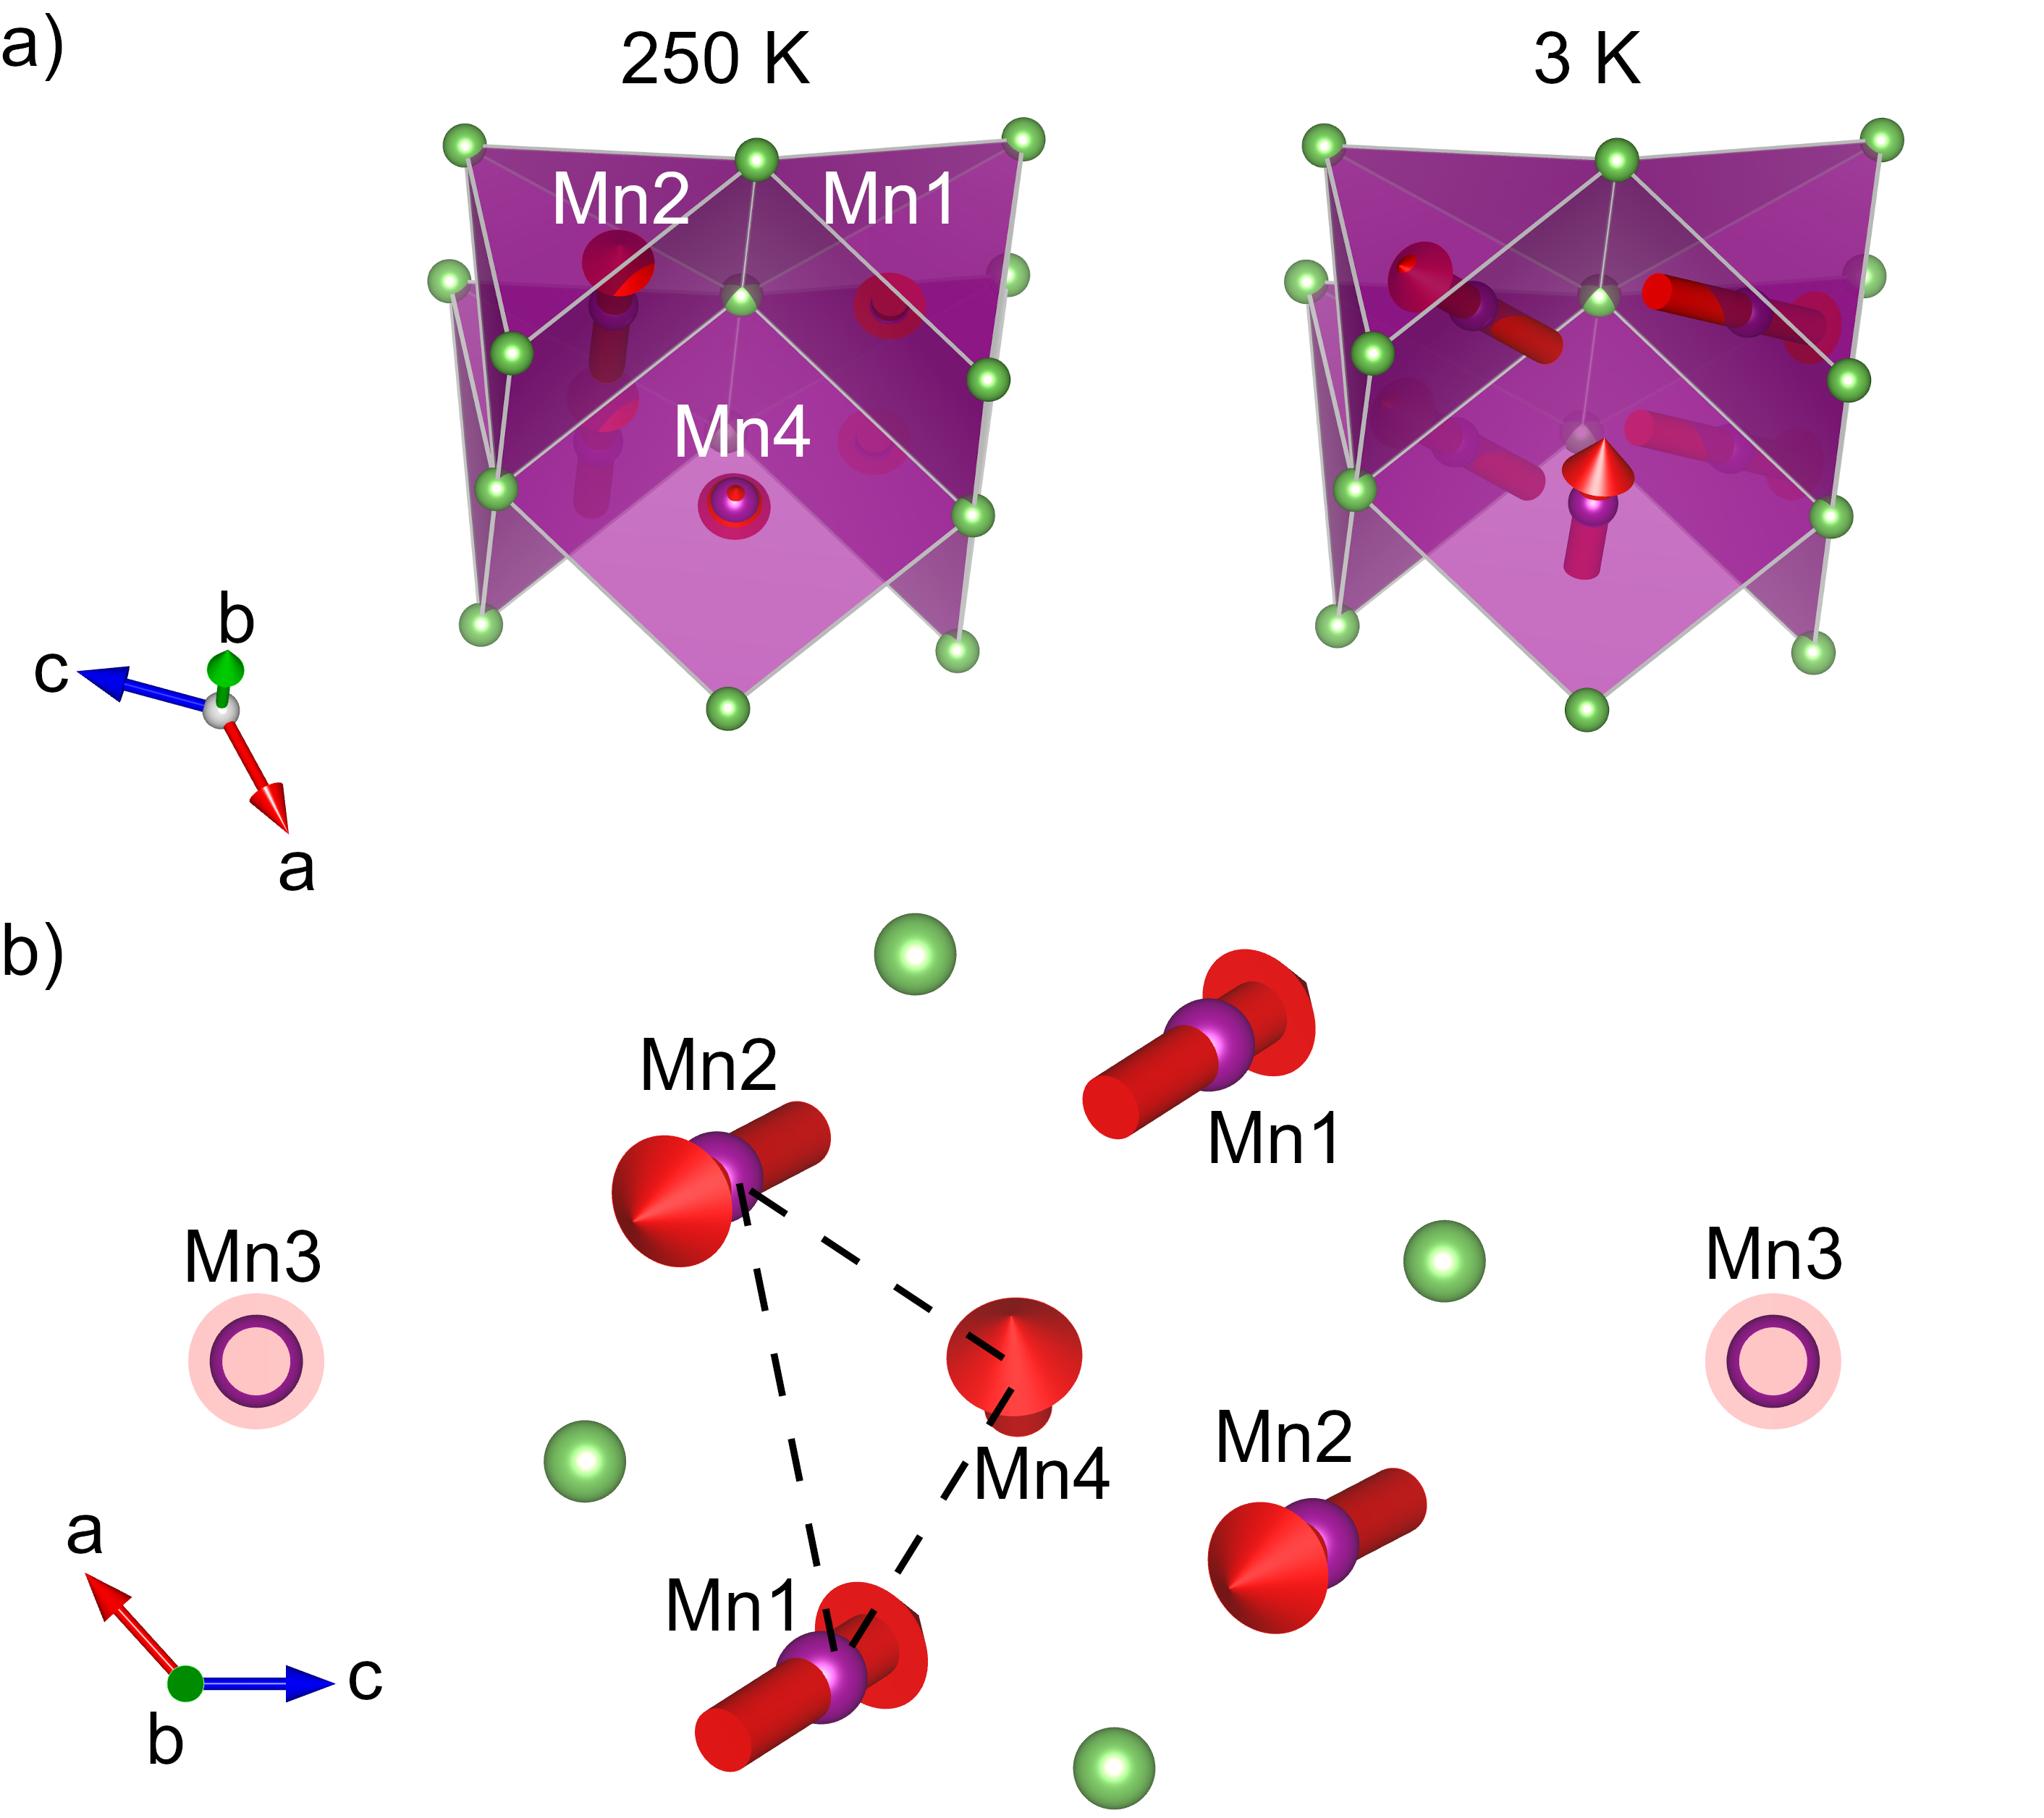
\includegraphics[width=\columnwidth]{figures/ch6/spin_canting_dps.png} \\
\caption{\label{fig:spin_canting}
Electronic band structure
}
\end{figure}

\begin{figure}
\centering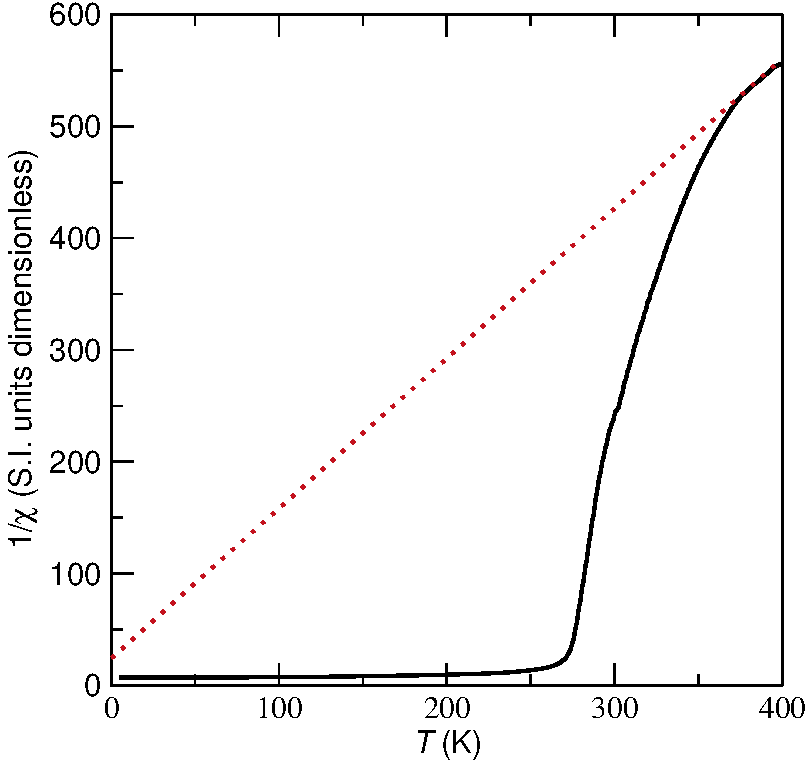
\includegraphics[width=\columnwidth]{figures/ch6/FC_52A_inverse_cropped.pdf} \\
\caption{\label{fig:inv_susceptibility}
Electronic band structure
}
\end{figure}

\Blindtext[6]

%chapter 7
\chapter{Spin canting in tetragonal CuMnAs}

\Blindtext[6]

%chapter 8
\chapter{Exchange interactions in Fe$_2$As probed by inelastic neutron scattering}

\begin{figure}
\centering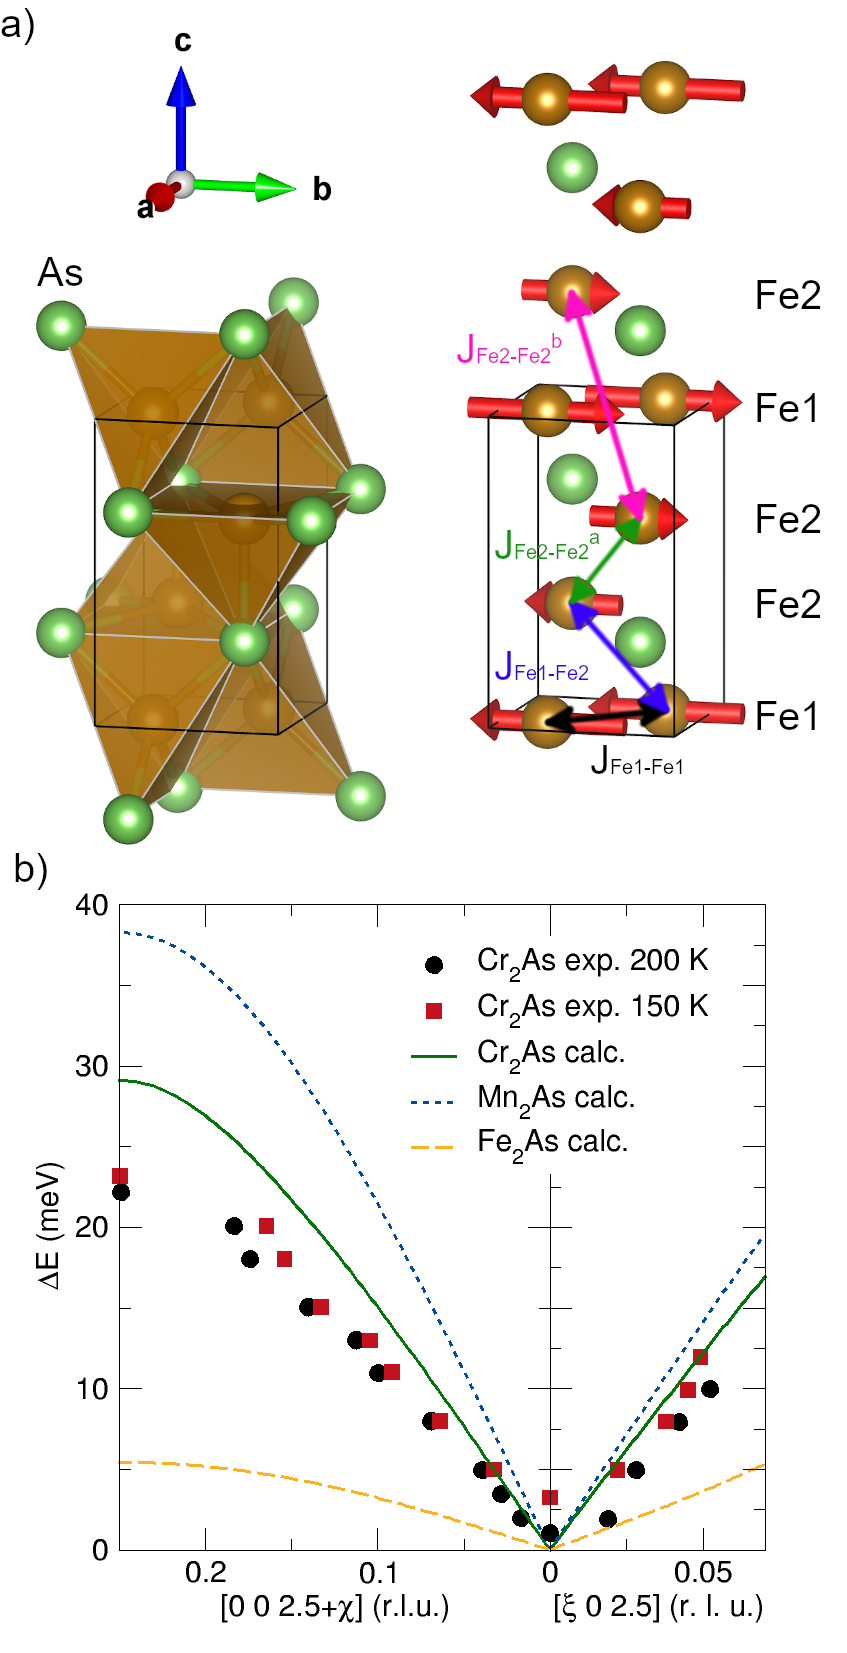
\includegraphics[width=0.5\columnwidth]{figures/ch8/Cr2As_INS_magnetic_structure.png} \\
\caption{\label{fig:Cr2As}
Electronic band structure
}
\end{figure}

\begin{figure}
\centering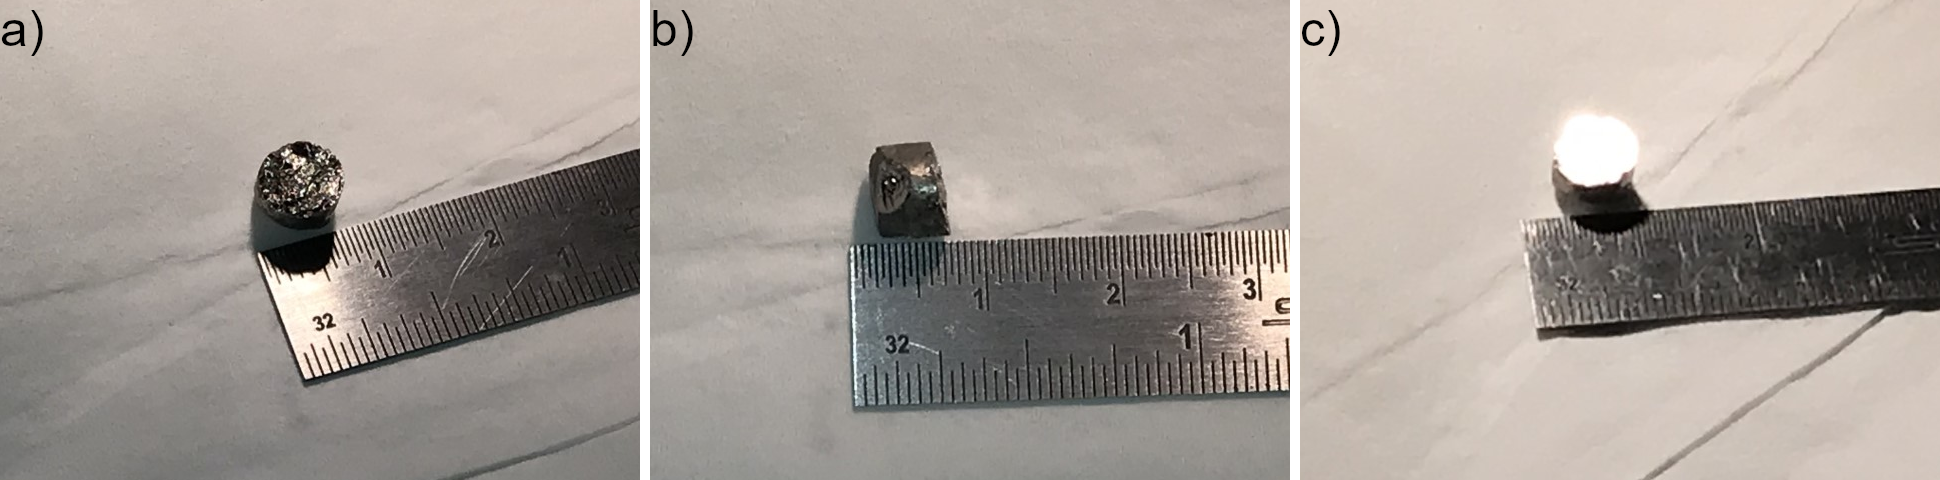
\includegraphics[width=\columnwidth]{figures/ch8/crystal.png} \\
\caption{\label{fig:crystal}
Electronic band structure
}
\end{figure}

\begin{figure}
\centering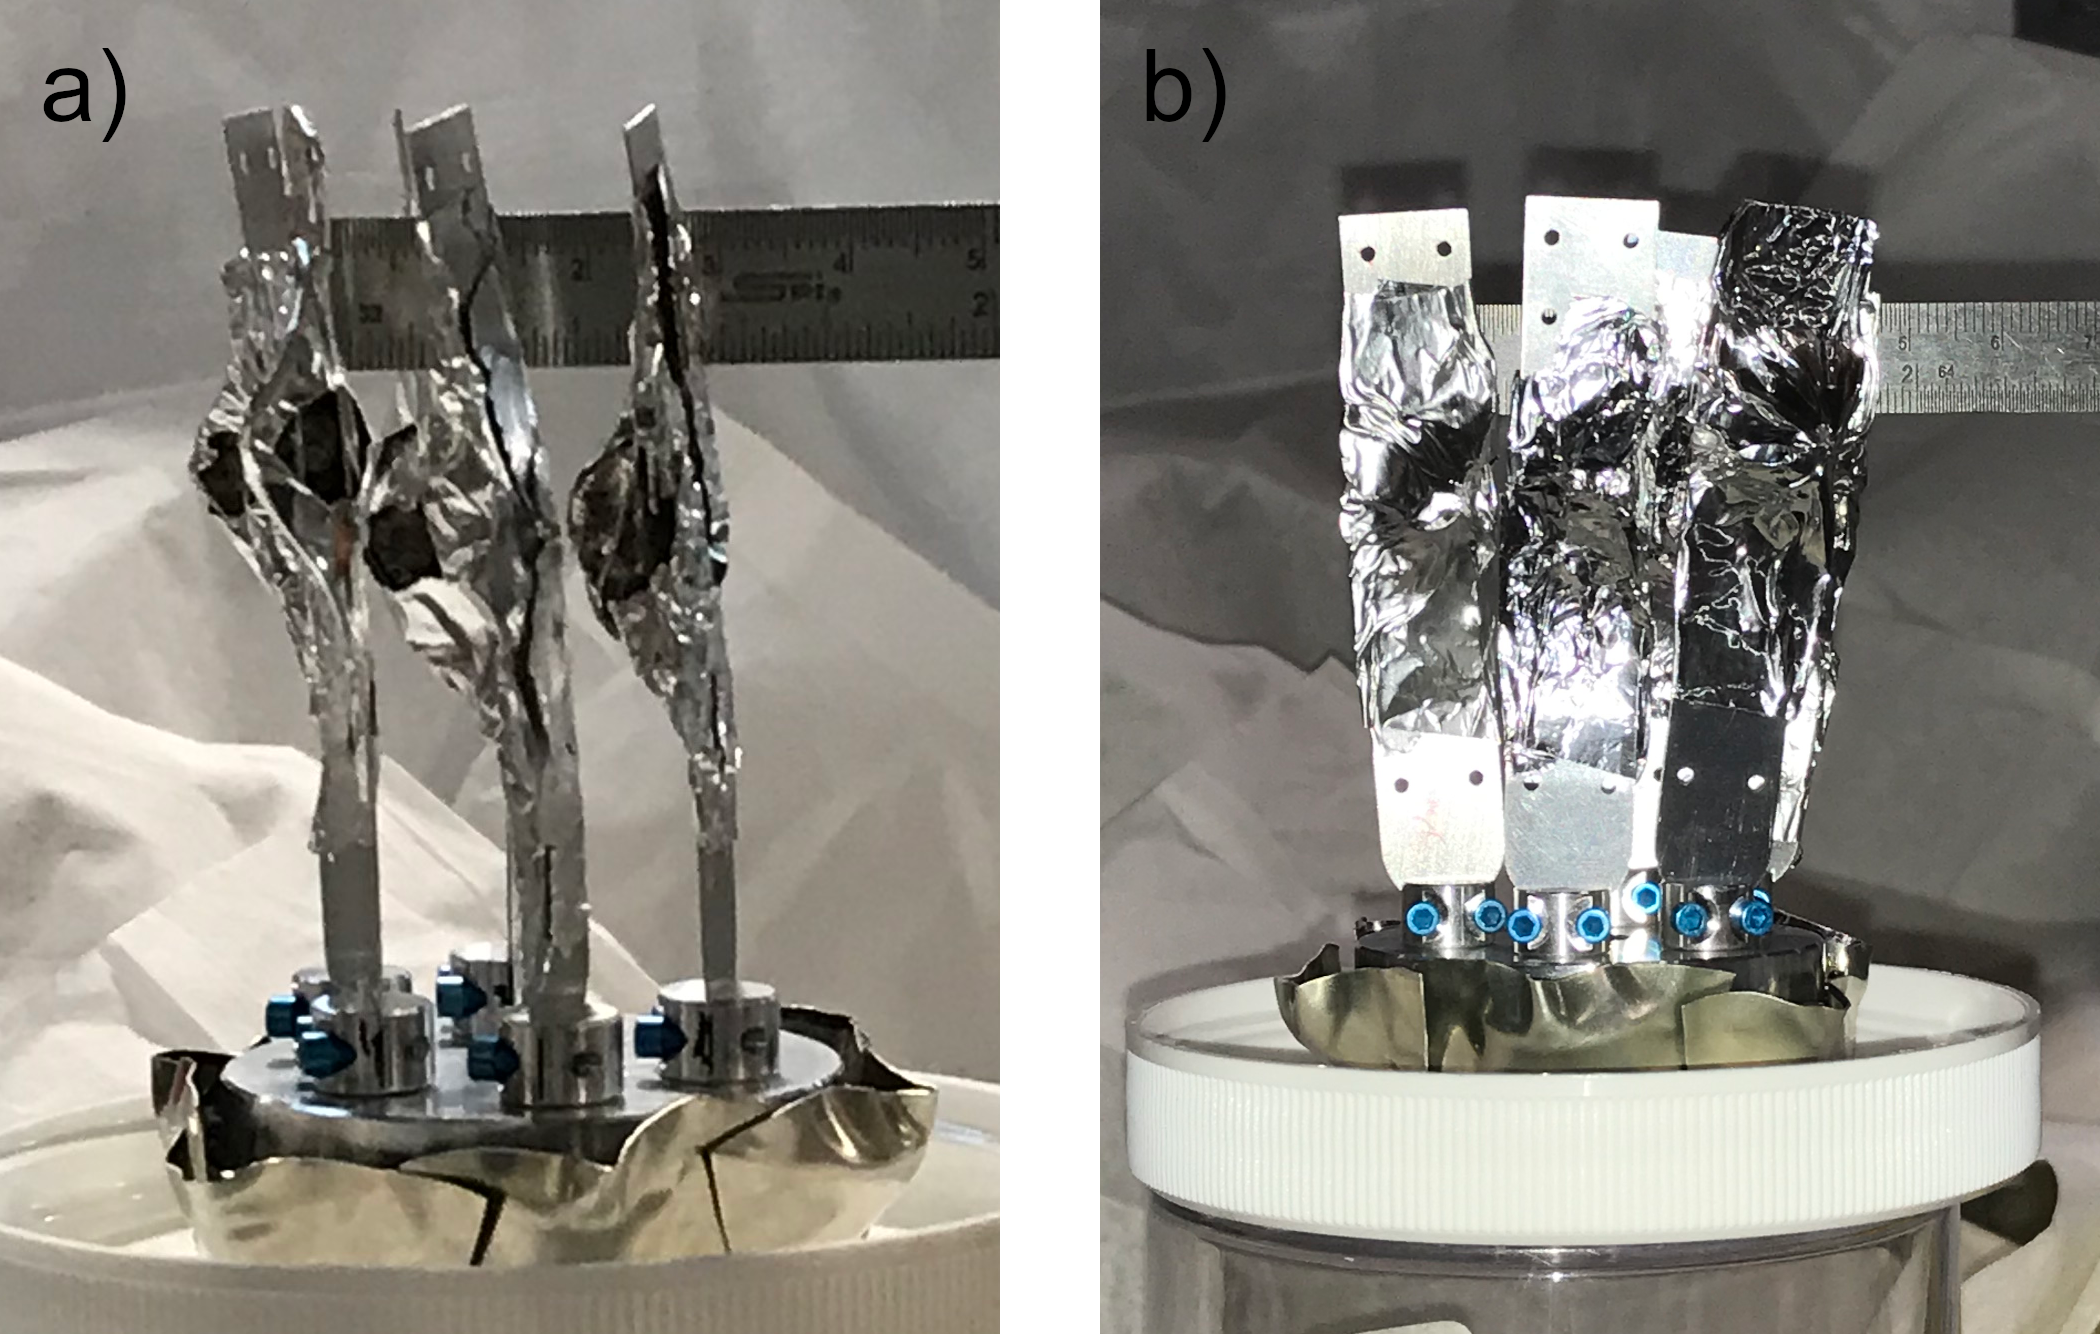
\includegraphics[width=\columnwidth]{figures/ch8/crystal_array.png} \\
\caption{\label{fig:crystal_array}
Electronic band structure
}
\end{figure}

\begin{figure}
\centering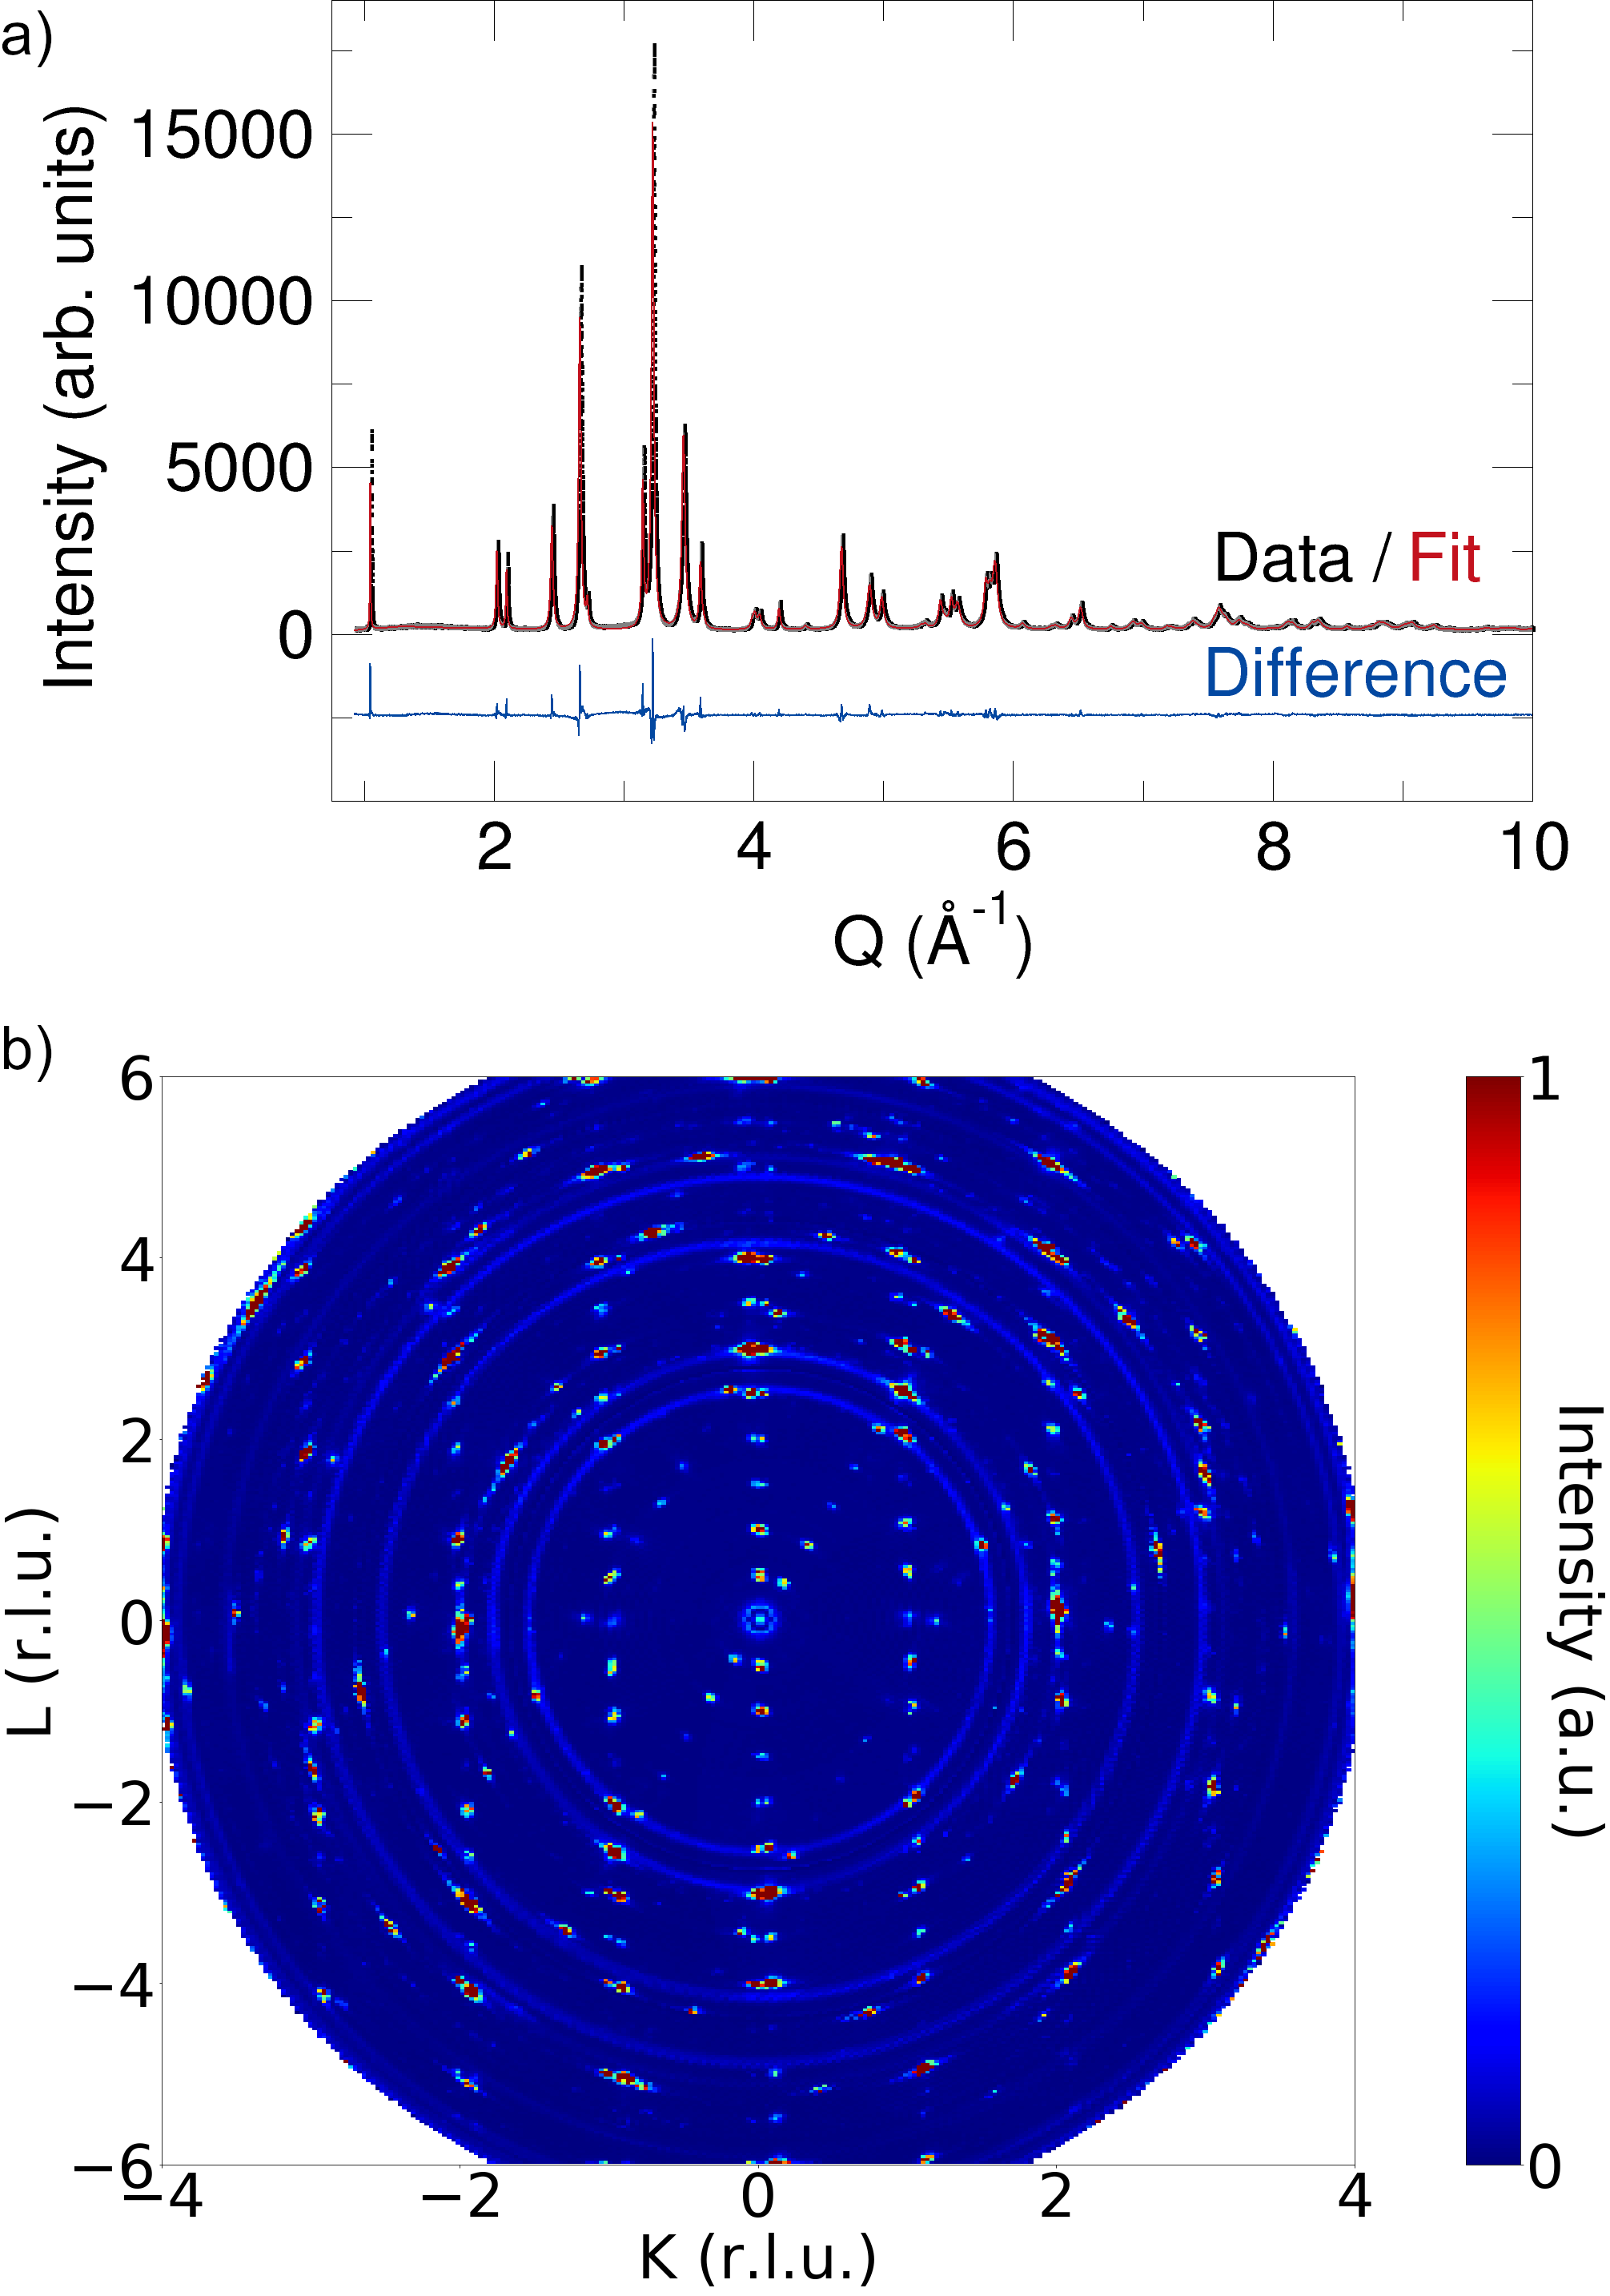
\includegraphics[width=\columnwidth]{figures/ch8/11BM_refinement_elastic_slice.png} \\
\caption{\label{fig:11BM_elastic_slice}
Electronic band structure
}
\end{figure}

\begin{figure}
\centering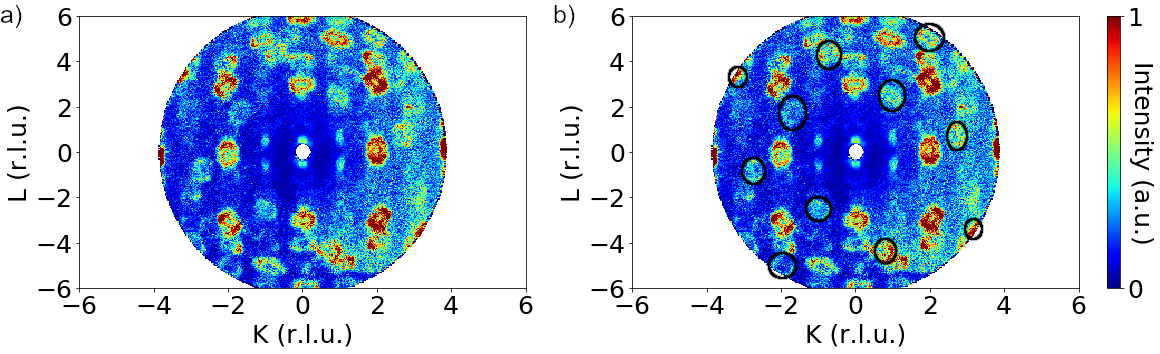
\includegraphics[width=0.7\columnwidth]{figures/ch8/suppl_misaligned_crystal_kl_slice.png} \\
\caption{\label{fig:misalign_crystal}
Electronic band structure
}
\end{figure}

\begin{figure}
\centering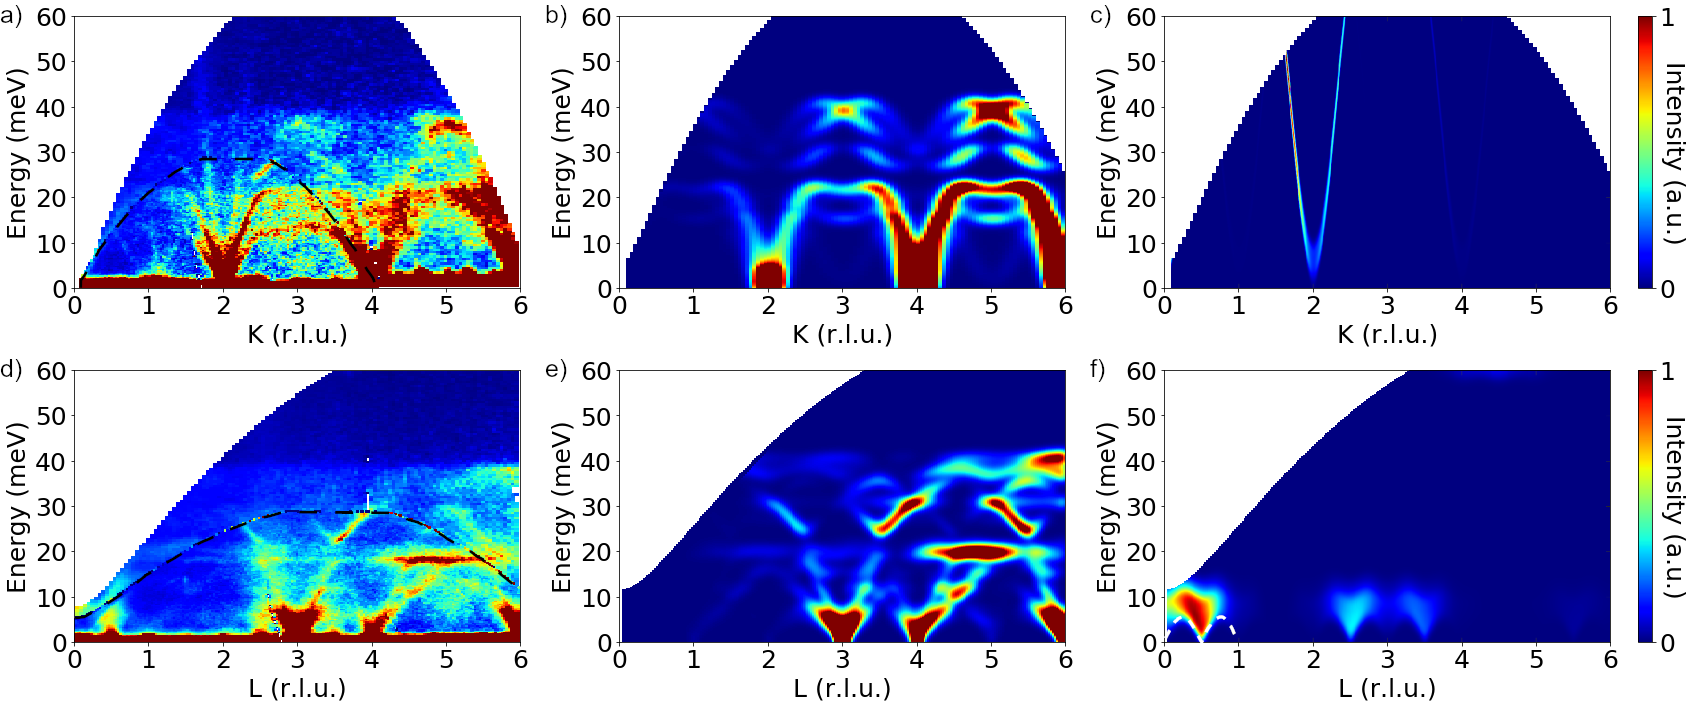
\includegraphics[width=\columnwidth]{figures/ch8/phonon_spectra_magnon_spectra_combined.png} \\
\caption{\label{fig:phonon_magnon_spectra}
Electronic band structure
}
\end{figure}

\begin{figure}
\centering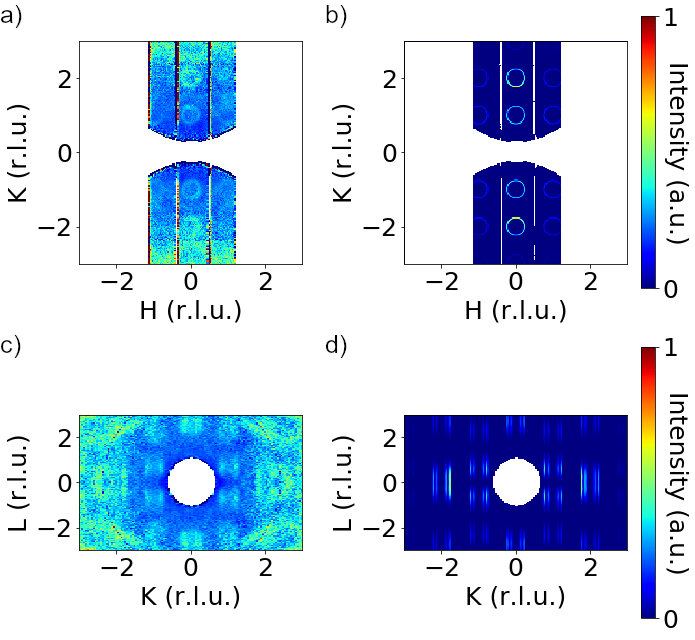
\includegraphics[width=\columnwidth]{figures/ch8/constant_energy_slices.png} \\
\caption{\label{fig:constant_energy_slices}
Electronic band structure
}
\end{figure}

\begin{figure}
\centering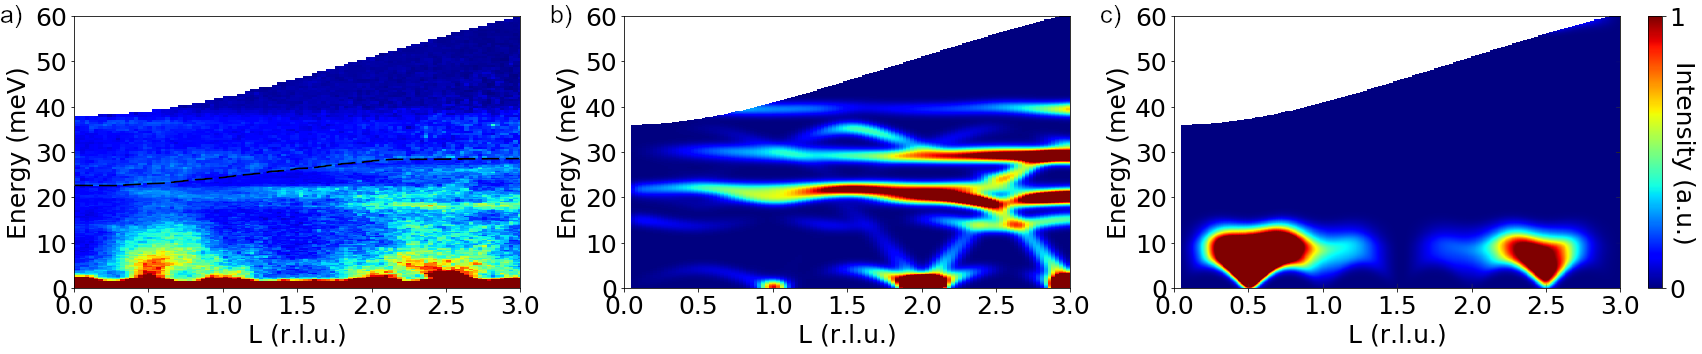
\includegraphics[width=\columnwidth]{figures/ch8/suppl_01L_INS_data.png} \\
\caption{\label{fig:01L_spectra}
Electronic band structure
}
\end{figure}

\begin{figure}
\centering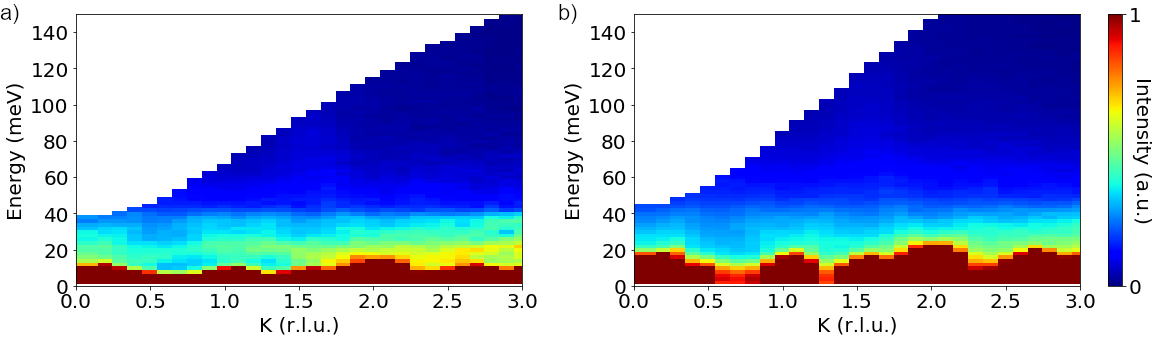
\includegraphics[width=\columnwidth]{figures/ch8/suppl_high_energy_data.png} \\
\caption{\label{fig:high_energy_data}
Electronic band structure
}
\end{figure}

\begin{figure}
\centering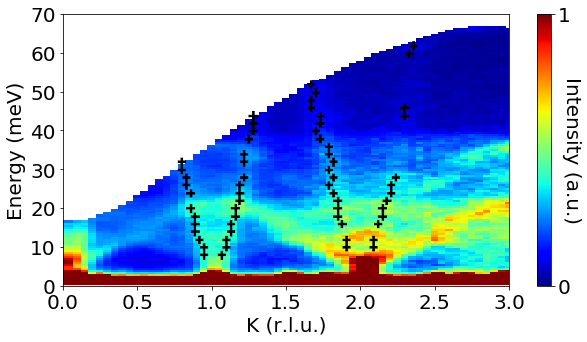
\includegraphics[width=\columnwidth]{figures/ch8/exp_data_points_0K0dot5.png} \\
\caption{\label{fig:exp_points}
Electronic band structure
}
\end{figure}

\begin{figure}
\centering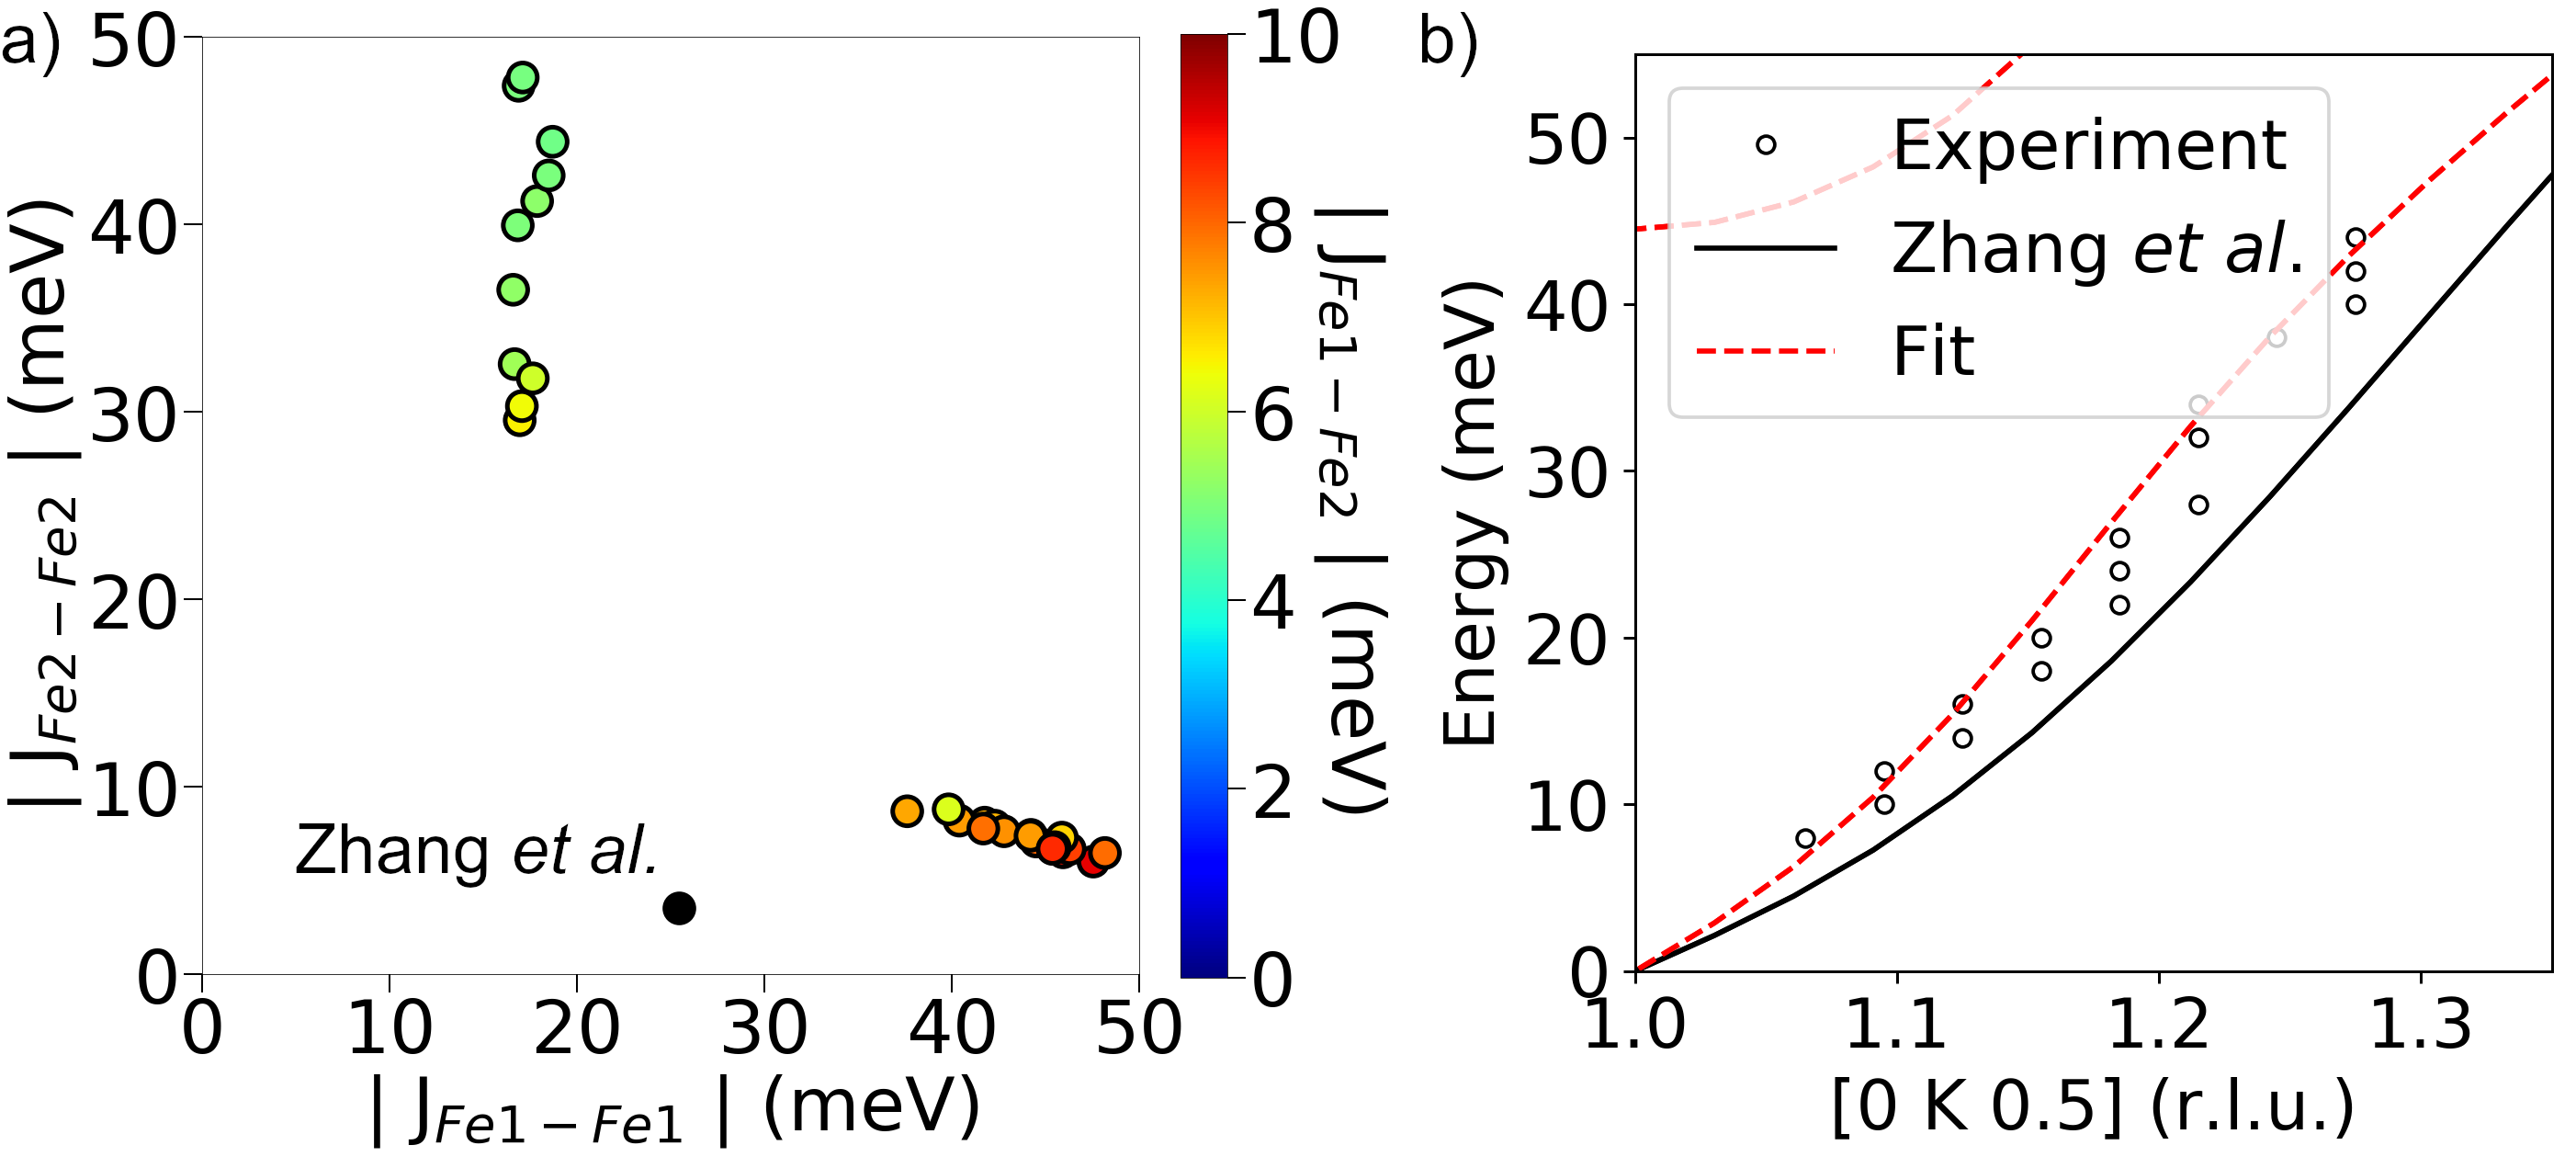
\includegraphics[width=\columnwidth]{figures/ch8/magnon_spectra_refinement.png} \\
\caption{\label{fig:refinement}
Electronic band structure
}
\end{figure}

\begin{figure}
\centering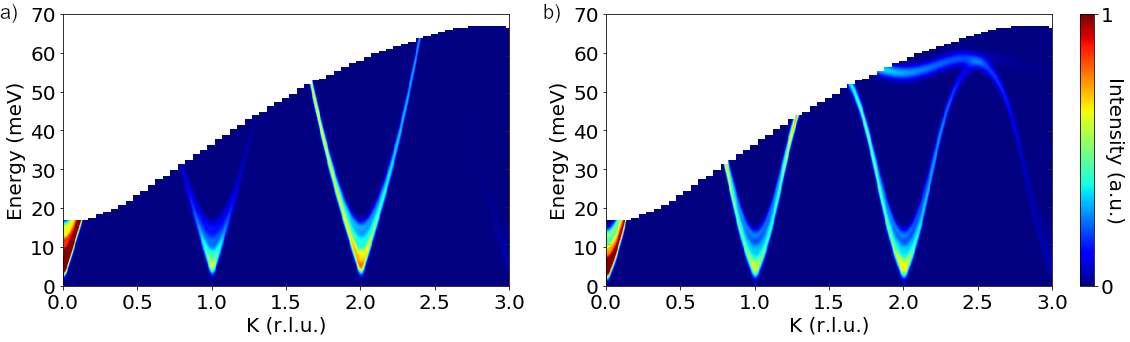
\includegraphics[width=\columnwidth]{figures/ch8/suppl_simulated_magnon_spectra_3J.png} \\
\caption{\label{fig:3J_fits}
Electronic band structure
}
\end{figure}

\Blindtext[6]

%chapter 9
\chapter{Conclusions}

\Blindtext[6]

\end{mainmatter}

% }}}

% {{{ back matter

\begin{backmatter}

\bibliographystyle{ieeetr}
\bibliography{thesis}

\end{backmatter}

%\appendix
%\chapter{My Appendix}

%\Blindtext[6]

% }}}

\end{document}
